% CREATED BY DAVID FRISK, 2016
% MODIFIED BY JAKOB JARMAR, 2016
% A few changes by Birgit Grohe, 2017 and 2018
% Adjustments with the help of Gustav Örtenberg 2019
% Parskip % bibliography system updated by Erik Ljungdahl, May 2022

% IMPORT SETTINGS
\documentclass[12pt,a4paper,twoside,openany]{report}
\input{include/settings/Settings}

\newcommand{\oneLineTitle}{Neural compression for multimodal Vehicle Data}

\newcommand{\multiLineTitle}[1]{Neural Compression \\[#1]  for Multimodal Vehicle Data}

\newcommand{\oneLineSubtitle}{Investigating different Architectures for Neural Compression Models for Multimodal Time Series Data}


\begin{document} 

% COVER PAGE, TITLE PAGE AND IMPRINT PAGE
\pagenumbering{roman}			% Roman numbering (starting with i (one)) until first main chapter
\input{include/frontmatter/Titlepage}

% ABSTRACT
\newpage
% CREATED BY DAVID FRISK, 2016
\oneLineTitle\\
\oneLineSubtitle\\
Tim Boleslawsky\\
Emrik Dunvald\\
Department of Computer Science and Engineering\\
Chalmers University of Technology and University of Gothenburg

\thispagestyle{plain}			% Supress header 
\section*{Abstract}
With the growing amount of data generated by modern vehicles, the need for edge efficient data processing and compression strategies becomes more apparent. As the amount of data grows so does the potential for machine learning models to extract insightful information from this data at later stages. Achieving high compression ratios while retaining only the essential components of the original data therefore becomes a the main goal of many compression strategies. Currently, the existing solutions for such a task on a resource constrained devices such as a vehicle are limited and often come with tradeoffs. This thesis investigates compression algorithms based on neural networks (commonly referred to as neural compression) which have shown promising results in other fields, such as image processing. Four neural codec architectures are explored and tested on industry relevant datasets with compression ratio, data reconstruction quality and downstream utility retention as the main metrics investigated.

% KEYWORDS (MAXIMUM 10 WORDS)
\vfill
Keywords: Signal Data, Time Series, Multimodal Data,Neural Compression, Edge Computing, Neural Codec, Autoencoder, Vector Quantization.

\newpage				% Create empty back of side
\thispagestyle{empty}
\mbox{}

% ACKNOWLEDGEMENTS
\newpage
% CREATED BY DAVID FRISK, 2016
\thispagestyle{plain}			% Supress header
\section*{Acknowledgements}
First, we would like to thank our supervisor, Yinan Yu, for her guidance and support throughout this project. Her feedback and insights were valuable for designing the thesis and overcoming challenges along the way. 

We would also like to thank the team at Volvo Group for providing technical support, access to their infrastructure and for their great support. In particular, we would like to thank our company advisor, Dhasarathy Parthasarathy, for his support and feedback on the project. We would also like to thank Szabolcs Torma and Alexander Bergersen for their help and support with technical matters and for providing feedback on the project.

Lastly, Tim would also like to thank his girlfriend Marie for always being there and always showing support. 

\section*{Disclaimer}
This thesis makes use of AI for spelling and grammar checking, as well as reformulating sentences for improved readability. The use of AI was limited to these tasks, and all content, including the structure and organization of the thesis, was created by the authors. The authors take full responsibility for the content of this thesis and any errors or inaccuracies that may be present.

\vspace{1.5cm}
Tim Boleslawsky, Gothenburg, \today \\
Emrik Dunvald, Gothenburg, \today

\newpage				% Create empty back of side
\thispagestyle{empty}
\mbox{}


% TABLE OF CONTENTS
\newpage
\tableofcontents

% OTHER FRONTMATTER
% List of figures (add to table of contents)
\clearpage
\phantomsection
\addcontentsline{toc}{chapter}{\listfigurename} 
\listoffigures
% List of tables (add to table of contents)
\clearpage
\phantomsection
\addcontentsline{toc}{chapter}{\listtablename}  
\listoftables


% START OF MAIN DOCUMENT
\clearpage
\setcounter{page}{1}
\pagenumbering{arabic}			% Arabic numbering starting from 1 (one)

% INTRODUCTION
% CREATED BY DAVID FRISK, 2016
\chapter{Introduction}
\label{chap:introduction}

Modern vehicles generate large amounts of telemetry data through distributed embedded systems, sensors, actuators, and in-vehicle networks~\cite{Lee2017,Navet2009,MITRE2023}. These systems are designed to support real-time functionality, but they are also constrained by limited communication bandwidth, storage capacity, and on-board compute resources~\cite{Navet2009}. In practice, this has led to the widespread use of event-triggered and threshold-based logging strategies, which reduce data volume by transmitting only selected events or diagnostic messages~\cite{AUTOSAR2022b,Navet2009}. While these approaches are effective for limiting network load, they also risk omitting information that may later be relevant for offline analysis or machine learning-based applications~\cite{Navet2009,EventDrivenDiagPatent}.

This challenge has become more important as vehicles generate increasingly rich signal-based data and as downstream machine learning tasks have become a central use of automotive telemetry~\cite{Bertoncello2021,Samantaray2023,Theissler2021}. Collected vehicle data is no longer used only for diagnostics or monitoring, but also for tasks such as predictive maintenance, anomaly detection, fleet analytics, and other forms of offline model training~\cite{Theissler2021,Oezdemir2024,Brunheroto2022}. For these use cases, data utility matters as much as data volume: aggressive reduction of telemetry may improve efficiency, but it can also degrade the performance of models trained on the resulting data~\cite{Tirupathi2022,Eichinger2015,Moon2018}. This creates a fundamental tension between efficient storage and transmission on the one hand and preserving task-relevant information on the other.

The theoretical basis for this tension comes from information theory and rate-distortion theory~\cite{Shannon1948,Shannon1949}. Information entropy describes how much uncertainty is contained in a signal and therefore provides an indication of how compressible that signal is~\cite{Shannon1948}. Rate-distortion theory extends this idea to lossy compression by formalizing the trade-off between bitrate and reconstruction quality~\cite{Shannon1949}. For machine learning settings, this trade-off is not sufficient on its own, because good reconstruction does not necessarily imply that the compressed representation is useful for downstream tasks~\cite{Marchioni2024,Cuza2024}. This is why modern learned compression methods are often framed in terms of autoencoders and information bottlenecks: they aim to produce compact latent representations while retaining the information that is relevant for later prediction or classification tasks~\cite{Yang2022,Tishby2000,Chen2023,Alemi2016}.

Within this thesis, neural compression is the central approach for addressing this problem. Neural compression methods use learned encoder-decoder architectures to transform high-dimensional input signals into more compact representations. In contrast to traditional algorithmic compression methods, these models can adapt to the structure of the data and can be optimized for the kinds of signals that occur in automotive telemetry~\cite{Yang2022,Zheng2023,Liu2024}. In particular, vector quantization offers a practical way to introduce discrete bottlenecks that reduce entropy while still allowing the model to preserve useful structure in the compressed representation~\cite{Yang2022,Hodo2025}. This makes neural compression especially attractive for edge-oriented settings, where the compressed data must be stored, transmitted, or processed under strict efficiency constraints~\cite{Azar2022,Hodo2025}.

Recent research shows that neural compression has been successful in a range of domains, including time-series, audio, speech, and other resource-constrained applications~\cite{Löhdefink2019,Zheng2023,Liu2024,Zeghidour2021,Defossez2022,Ji2025,Azar2022,Hodo2025}. For time-series data, continuous-latent autoencoder approaches have demonstrated strong reconstruction performance, while vector-quantized methods such as EdgeCodec show that lightweight discrete compression can be effective in edge-deployment scenarios~\cite{Zheng2023,Hodo2025}. At the same time, the literature also shows that many methods primarily optimize reconstruction error, whereas downstream task utility is often treated as secondary or is not investigated in depth~\cite{Zheng2023,Hodo2025}. For vehicle telemetry, this is a crucial limitation, because a representation that reconstructs well is not necessarily the best representation for predictive maintenance or anomaly detection~\cite{Theissler2021,Oezdemir2024,Tirupathi2022}.

The background of this thesis therefore combines three strands of work: the properties and constraints of automotive telemetry, the information-theoretic foundations of compression, and the recent development of neural compression methods. Taken together, these areas motivate the central question of the thesis, namely how to compress multimodal vehicle telemetry in a way that remains useful for downstream machine learning tasks while still achieving meaningful compression and efficiency gains. The following sections build on this background by stating the concrete aim of the thesis, defining the research questions, and outlining the limitations of the study.

\section{Aim}
The aim of this thesis is threefold. First, two existing neural compression methods are applied to automotive and IoT time-series data in order to evaluate how they perform in terms of compression ratio, reconstruction quality, and computational efficiency. One of these methods is based on vector quantization, while the other serves as a continuous-latent baseline.

Second, the compressed representations produced by these methods are used to train downstream machine learning models and are compared against models trained on uncompressed data. This makes it possible to assess how much task-relevant information is retained after compression and reconstruction.

Third, the two methods are further explored through changes to the quantization strategy and loss function. The goal of this exploratory part is to investigate whether reconstruction loss and downstream utility retention can be improved further without sacrificing the general compression objective and computational efficiency.

\section{Research Questions}
This thesis is guided by the following research questions:

\begin{enumerate}
	\item RQ1: How do the selected neural compression methods perform on automotive and IoT time-series data in terms of compression ratio, reconstruction quality, and computational efficiency?
	\item RQ2: To what extent do downstream machine learning models trained on reconstructed compressed data retain task performance compared to models trained on uncompressed data?
	\item RQ3: Where do the existing neural compression methods fall short in terms of reconstruction quality and downstream utility retention, and which quantization strategies and loss functions can mitigate these limitations?
\end{enumerate}

\section{Limitations}
Due to time constraints and the scope of this thesis, there are several limitations to the work presented. 

First, the work forgoes testing on real hardware as that is very time consuming and difficult to set up while contributing relatively little to the main research question. Instead, canonical methods to measure computational efficiency are employed. 

The work is further limited to testing only regression tasks and anomaly detection as downstream tasks due to time constraints and the structure of the available datasets. These two tasks should, however, be a good representation of common downstream tasks, and adding more tasks would likely not drastically change the conclusion of the thesis. 

To keep the compressed data representation as versatile as possible, no task-aware compression techniques are implemented. While task-aware compression could potentially yield better performance for specific tasks, it would limit the generalizability of the compressed representation and add significant complexity to the work. It also results in a more relevant comparison to other compression techniques which are not task-aware. 


% This chapter presents the section levels that can be used in the template. 

% \section{Section levels}
% \autoref{tab:sections} presents an overview of the section levels that are used in this document. The number of levels that are numbered and included in the table of contents is set in the settings file \texttt{Settings.tex}. The levels are shown in Section \ref{Section_ref}.

% This is a new paragraph and should have proper parskip or indentation. Don't forget to cite your sources~\cite{Brajnik2008}. % '~' becomes space which cannot line break.

% \begin{table}[h]
% \centering
% \caption{Section levels} % Table text above table.
% \begin{tabular}{ll} \hline
% Name & Command\\ \hline
% Chapter & \textbackslash\texttt{chapter\{\emph{Chapter name}\}}\\
% Section & \textbackslash\texttt{section\{\emph{Section name}\}}\\
% Subsection & \textbackslash\texttt{subsection\{\emph{Subsection name}\}}\\
% Subsubsection & \textbackslash\texttt{subsubsection\{\emph{Subsubsection name}\}}\\
% %Paragraph & \textbackslash\texttt{paragraph\{\emph{Paragraph name}\}}\\
% %Subparagraph & \textbackslash\texttt{paragraph\{\emph{Subparagraph name}\}}\\ \hline\hline
% \end{tabular}
% \label{tab:sections}
% \end{table}

% \section{Section} \label{Section_ref}
% \subsection{Subsection}
% \subsubsection{Subsubsection}
% %\paragraph{Paragraph}
% %\subparagraph{Subparagraph}



% Background
% CREATED BY DAVID FRISK, 2016
\chapter{Background}
\label{chap:background}

% 2.0 Short Introduction to Theory Chapters - Outline the structure of these chapters and the purpose for each. 
This section introduces necessary context for further discussion within this thesis. The in-vehicle system and related components will be introduced, followed by an introduction to modern challenges in regard to data processing and data usage in the automotive industry. The purpose of this chapter is to provide the necessary background for the reader to understand the motivation and relevance of the research presented in this thesis. It also serves to establish a common understanding of key concepts and terminology that will be used throughout the thesis.

% 3.1 In-Vehicle Systems and Event-Triggered Logging - DONE (TIM) - DONE (EMRIK)
\section{In-Vehicle Systems and Event-Triggered Logging}

\textbf{The In-Vehicle Embedded System} An embedded system is a computer system integrated into a physical device or product to perform a dedicated function as part of a larger system~\cite[pp.~vii--x,~1--3]{Lee2017}. The in-vehicle embedded system is a specialized embedded system integrated within a vehicle. It is essential for real-time functions like controlling, monitoring, and enhancing various automotive operations~\cite[pp.~1-1--1-5]{Navet2009}. These in-vehicle embedded systems, like embedded systems in general, typically consist of both hardware and software components, such as electronic control units (ECUs), sensors, actuators, and communication interfaces~\cite[pp.~3--4]{Lee2017},~\cite[pp.~1-3--1-10]{Navet2009}. 

ECUs serve as the primary processing nodes in in-vehicle embedded systems. They are responsible for executing control algorithms on sensor inputs and issuing commands to actuators. They also handle local control logic while coordinating via in-vehicle networks to form a distributed system~\cite[pp.~1-8--1-19]{Navet2009}. An example of how ECUs work together to create the in-vehicle embedded system is illustrated by~\cite[pp.~1-8--1-9]{Navet2009}. In the example an ECU coordinates a request, e.g., locking or unlocking a door, while the controller realize the request on the physical system, which is controlled by another ECU\@. The resulting system is the main generator of telemetry data within the vehicle. Vehicle telemetry data, usually defined as data that is produced by the vehicle and sent off-board, is key to improving important aspects of these vehicles like safety~\cite[pp.~1--5]{MITRE2023}. This vehicle telemetry data is at the core of this thesis.

\textbf{In-Vehicle Networks} As mentioned above, in-vehicle networks serve as the connectors between the ECUs of the in-vehicle embedded system. 
Among these in-vehicle networks Control Area Networks (CAN), Local Interconnect Networks (LIN), FlexRay, and Ethernet are popular representatives that enable efficient communication and coordination among different vehicle subsystems~\cite[pp.~1-2--1-5]{Navet2009}. 

From a technical perspective, ECUs connect to these networks via dedicated communication services. The communication services are tasked with providing a uniform interface to the network, while hiding protocol and message properties from the application~\cite[p.~48]{AUTOSAR2022}. The in-vehicle network protocols are categorized into three classes, A, B, and C. LIN falls into category A with a bit rate below 10 kbps and application in sensor and actuator networks. CAN-B is a representative of category B with a bit rate between 10--500 kbps. Category B networks serve vehicle-centric domains and body electronics. Category C in-vehicle networks like FlexRay or CAN-C are defined by having a bit rate of lower than 1 Mbps and used in safety-relevant systems~\cite[pp.~1-12--1-13]{Navet2009}. Despite their effectiveness in their respective use-cases, all in-vehicle networks must contend with fundamental bandwidth limitations that constrain data throughput across the vehicle~\cite[pp.~1-18--1-19]{Navet2009}.

\textbf{Event-Triggered and Time-Triggered Logging} Event-triggered logging and diagnostic frameworks, which record data only when specific error codes occur or threshold crossings are detected, are widely adopted to reduce data transmission and avoid bus saturation in complex systems such as the in-vehicle embedded system~\cite[pp.~7--13]{AUTOSAR2022b}. According to the AUTOSAR Diagnostic Log and Trace (DLT) standard, this mechanism can be implemented as follows: When software components or Basic Software modules report errors via the Default Error Tracer, the DLT module receives these via a specified function and stores timestamped log/trace messages to flash storage~\cite[p.~25]{AUTOSAR2022b}. Non-critical events are filtered during normal operation~\cite[pp.~30--35]{AUTOSAR2022b}. 

Time-triggered logging serves as an alternative to event-triggered logging and works by setting predetermined points in time where data is transmitted. The validity of this strategy is easily monitored, as the time-frame scheduling is predictable and missing messages are immediately identified~\cite[pp.~4-5]{Navet2009}. Although Navet discusses these paradigms in the context of communication scheduling, similar principles apply to diagnostic event- and time-based mechanisms, which leads to similar struggles in these systems.

While these approaches have been effective in reducing the data load of the in-vehicle networks, they come with major limitations. Two immediate issues these diagnostic frameworks struggle with is presenting an unbiased and comprehensive monitoring of the system, while having to carefully tune event thresholds and diagnostic parameters~\cite[pp.~4-5--4-6]{Navet2009},~\cite{EventDrivenDiagPatent}. In the next section we will go further into how these limitations are accentuated by recent developments. 

% 3.2 Downstream ML Tasks and Data Quantity - DONE (TIM) - DONE (EMRIK)
\section{Downstream Machine Learning Tasks and Data Quantity}\label{sec:downstream-ml-and-dq} 

Two developments in recent years further underline the shortcomings of event-triggered logging in automotive systems: the massive increase in signal-based data in the in-vehicle network and the growing relevance of downstream machine learning (ML) tasks. 

\textbf{Data Quantity in Modern Vehicles} Recent industry and research reports indicate that the data quantity generated by sensors and the amount of interconnectivity in vehicles is growing at an extremely rapid pace. According to a 2021 automotive electronics report, by 2030, about 95\% of new vehicles will be connected, up from around 50\% today~\cite{Bertoncello2021}. Another report states that even today, a single car can generate up to 1 terabyte (TB) of data per hour from its sensors~\cite{Samantaray2023}. This explosive growth is driven by the increasing number and sophistication of sensors—such as cameras, radars, and lidars—required for advanced safety and autonomous driving features, with the complexity and volume of data presenting significant challenges for storage, processing, and transmission within embedded automotive systems~\cite{Samantaray2023},~\cite[pp.~3--5]{Komorkiewicz2023}. While much of the focus in research and reporting on this issue centers on autonomous driving technologies like lidars and cameras, it is important to note that the core of the in-vehicle system, the ECU, is also a major contributor to the data quantity issue. This implies that not only autonomous driving technologies but modern vehicles in general are facing these challenges~\cite[pp.~3--4]{Komorkiewicz2023}.

\textbf{Downstream ML Tasks} Modern vehicles increasingly rely on data-driven intelligence to enhance safety, reliability, and efficiency. As there currently exist no conclusive definition of these tasks, we will refer to them as downstream ML tasks within the context of this thesis. These downstream ML tasks we define as the offline use of collected vehicle data for the training of ML models for various tasks. This is distinctly different from real-time perception and control systems. Downstream ML tasks have become central to automotive-system design. Theissler et al.~\cite[p.~2]{Theissler2021} mention three reasons for the rise of importance of these downstream ML tasks: data availability, breakthroughs in algorithm development and the advancements in computational power. Prominent examples of downstream ML tasks in the automotive context include: Predictive maintenance tasks aim to predict the expected time of a failure, thereby helping to estimate remaining functionality of components or systems~\cite[p.~3]{Theissler2021}. Anomaly and intrusion detection tasks want to find anomalies or outliers in data points which is especially relevant in fragile systems like the CAN network~\cite[pp.~1--3]{Oezdemir2024}. Fleet-level management operations like fuel consumption that aim to better utilize important assets in vehicle systems~\cite[pp.~1--2]{Brunheroto2022}. Utility loss in the datasets used to train the models for these tasks translates directly to degraded model performance, increased operational costs, and missed business opportunities~\cite[pp.~4--5]{Komorkiewicz2023}. This further underlines the importance of a comprehensive data logging strategy.

There exists relatively little research on the use of event-triggered logging systems as a compression strategy and it's impact on downstream ML tasks. It is therefore difficult to definitively say that event-triggered logging systems specifically produce data with lower utility. Studies have however shown that similar utility agnostic data reduction strategies can have negative impacts on downstream utility in the domain of time-series data. One such example comes from a study by~\cite{Tirupathi2022} where the authors show that a 10-minute aggregation of the data leads to degraded utility for downstream ML tasks. In this specific case, the F1-score of the predictive downstream model was reduced by from 0.63 to 0.50 when trained on the aggregated data compared to the original dataset. The same study also shows that a model based lossy compression technique can be implemented without significant utility loss which suggests that more strategic data reduction techniques can retain more utility for downstream ML tasks. Further analysis of the impact of lossy compression algorithms on time series task utility in general has been done by~\cite{Eichinger2015} and~\cite{Moon2018}. It is important to note, that, while challenging, at specific error bounds compression techniques within these studies can actually show improvement to the task metrics. All this highlights the need for a strategic lossy compression technique that accounts not only for reconstruction, but also for downstream task utility. 

\section{Related Work}

\textbf{Time-Series Neural Compression} Neural compression for time-series data has been studied, but many methods are not optimized for edge deployment. The architecture proposed by Zheng and Zhang~\cite{Zheng2023} is representative of this line of work. Their method uses a continuous-latent autoencoder with recurrent modules and is primarily optimized for reconstruction quality, while computational efficiency and downstream task utility retention are not central optimization targets~\cite{Zheng2023}.

\textbf{Edge-Optimized Neural Compression} The majority of research labeled as ``edge-optimized neural compression'' focuses on compressing ML models for deployment rather than compressing input data. Lai et al.~\cite{Lai2026} highlight the importance of enabling complex deep learning models on resource-constrained edge devices. Key developments include improved efficient transformer variants and knowledge-distillation methods~\cite{Lai2026}. These advances address one side of the edge-optimization problem (model compression), while the complementary side is efficient compression of the data itself. EdgeCodec is a notable example of this latter direction and is discussed below.

\textbf{Audio/Speech Neural Compression} The audio/speech community contains extensive research on neural compression, with a strong emphasis on vector quantization. A key development in this literature is residual vector quantization (RVQ). RVQ works by layering hierarchical quantizers whith each layer quantizing the residuals of the previous layer~\cite[pp.~495--507]{Zeghidour2021}.

\begin{itemize}
    \item SoundStream (Google, 2021): first major use of RVQ for audio compression~\cite[pp.~495--507]{Zeghidour2021}.
    \item EnCodec (Meta, 2022): refined RVQ for high-quality audio~\cite{Defossez2022}.
    \item WaveTokenizer (2024): recent RVQ-based audio codec~\cite{Ji2025}.
\end{itemize}

\textbf{EdgeCodec} EdgeCodec transfers RVQ ideas from audio/speech processing to time-series compression (aerospace sensor data) and is explicitly designed for edge deployment. This is achieved through a lightweight encoder deployed on the edge and a heavier decoder executed in the cloud~\cite{Hodo2025}. As a result, EdgeCodec is a notable outlier in neural compression literature and addresses many challenges apparent in the research field. However, it has important limitations for the present use case. For one, EdgeCodec is optimized for smooth, continuous aerospace sensor streams rather than mutlimodal vehicle telemetry. And second, EdgeCodec focuses on reconstruction error and omits analysis of downstream task utility retention.

The literature review indicates that neural compression, VQ-based quantization, and lightweight design principles have all been explored individually. The remaining gap is a method tailored to mutlimodal data that explicitly optimizes downstream ML task utility rather than reconstruction quality alone. Based on this gap, the present thesis evaluates two existing solutions, namely the continuous-latent autoencoder by Zheng and Zhang~\cite{Zheng2023} and EdgeCodec~\cite{Hodo2025}, with respect to reconstruction quality on multimodal data and downstream ML task performance. Baseline models derived from these works are implemented and evaluated on automotive and IoT telemetry data, with the objective of identifying and improving design choices for multimodal data and downstream utility retention.


% THEORY
% CREATED BY DAVID FRISK, 2016
\chapter{Theory}
\label{chap:theory}

This section provides the theoretical background necessary to understand the research presented in this thesis. It covers the fundamental concepts of information theory, compression theory, and neural compression, as well as the specific architectures used as baselines in this work. The goal is to establish a solid theoretical foundation for the subsequent empirical evaluations and proposed improvements.

% 2.3 Compression Theory and Traditional Methods - DONE (TIM) - DONE (EMRIK)
\section{Compression Theory and Traditional Methods}

\textbf{Information Theory} Because information theory provides the basis for compression methods, its core concepts are introduced here before discussing compression itself. Entropy is key to information theory. It measures the uncertainty of a random variable and is computed from its probability distribution. More specifically, the uncertainty in a probability distribution is the expected negative log-probability of its outcomes. The entropy of a discrete distribution $p = {(p_i)}_i$ is defined as \[H(p) = -\sum_i p_i \log p_i,\] where the base of the logarithm determines the unit~\cite{Shannon1948}.

To illustrate with a weather example, suppose the true probabilities of ``rain'' and ``shine'' are $p_1 = 0.3$ and $p_2 = 0.7$, respectively. Then (using base-2 logs), \[H(p) = -(p_1 \log p_1 + p_2 \log p_2) \approx 0.61.\] Suppose the measurements are instead from Abu Dhabi, where the probabilities might be $p_1 = 0.01$ and $p_2 = 0.99$. The entropy is now approximately $0.06$. There is thus much less uncertainty about any given day compared to a place where it rains 30\% of the time. In this way, information entropy quantifies the inherent uncertainty in a distribution of events.

Entropy is central to compression because it indicates how compressible data is. High-entropy data is less predictable and therefore harder to compress, while low-entropy data has redundant patterns and is therefore easier to compress~\cite{Shannon1948}.

The other important information theory concept to understand in the context of compression is mutual information. Mutual information, formally defined as $I(X;Y)$ answers the question ``How much does one variable tell me about another?''~\cite{Shannon1948}.

\textbf{Compression} Compression, as originated in information theory by Shannon~\cite{Shannon1948}, is the process of encoding information using fewer bits than the original representation. Compression techniques can be broadly categorized into lossless and lossy methods. Lossless compression is based on two principles: distribution modeling, sometimes called entropy modeling, and entropy coding. Entropy modeling involves creating a probabilistic representation of the data, while entropy coding assigns shorter codes to more frequent symbols based on their probabilities, thereby minimizing the average code length. Entropy serves as the lower bound (in bits per symbol) for any lossless compression scheme. Lossy compression on the other hand allows for some loss of information in exchange for a higher rate of compression. This is typically achieved through techniques such as transform coding and quantization~\cite{Sayood2017}. The compression ratio (CR) is key to lossy compression methods, and is defined as the size of uncompressed data divided by the size of compressed data~\cite{Thomasian2022}. For the purpose of this thesis, the focus will be on lossy compression as this is more suitable for common downstream ML tasks where some loss of fidelity is acceptable as long as the relevant information for the task is preserved.

\textbf{Rate-Distortion Theory} Rate-distortion theory provides the fundamental framework for lossy compression, quantifying the minimum bitrate $R(D)$ required to represent data with acceptable distortion at most $D$. Building on entropy and mutual information introduced earlier, it formalizes the fundamental tradeoff between rate and fidelity central to lossy compression. The rate-distortion function is formally defined as \[R(D) = \min_{p(\hat{X}|X):\ E[d(X,\hat{X})] \leq D} I(X;\hat{X}),\] where $d(x,\hat{x})$ is a distortion measure, e.g., squared error, $E[\cdot]$ is the average over all data points or expectation, and the minimum bitrate is computed over all distributions $p(\hat{X}|X)$ achieving average distortion at most $D$. Shannon's rate-distortion theorem proves this isn't just a theoretical lower bound and practical codes exist that get arbitrarily close to $R(D)$ bits/symbols while keeping distortion below $D$.~\cite{Shannon1949}.

Distortion measures quantify the cost of representation between original data $X$ and its compressed reconstruction $\hat{X}$. They are essential in rate-distortion theory, where the goal is to minimize bitrate subject to $E[d(X,\hat{X})] \leq D$ for a chosen distortion threshold $D$. Widely used examples for distortion measures include the squared error (MSE) or the Hamming distance. MSE is defined as $d(x,\hat{x}) = {(x - \hat{x})}^2$, and is often used for numerical/time-series data due to its mathematical tractability. The Hamming distance on the other hand is defined as $d(x,\hat{x}) = \sum_i \mathbf{1}\{x_i \neq \hat{x}_i\}$, and is used for binary or categorical data~\cite[pp.~304--305]{Cover2006}.

In the ML context, particularly in automotive systems, or in fact IoT systems in general, rate-distortion analysis denotes the trade-off between efficiently handling large quantities of data and maximizing model performance. So in this sense, rate-distortion theory gives the theoretical framework to the downstream ML task challenges described in Section~\ref{sec:downstream-ml-and-dq}. Traditional lossy compression techniques can reduce data volume, but often at the cost of losing critical information necessary for accurate ML tasks such as predictive maintenance, anomaly detection, and fleet analytics~\cite{Marchioni2024}. The impact of this trade-off is well-documented in the literature. Cuza et al.~\cite{Cuza2024} for example, study the impact of lossy compression techniques on time series forecasting tasks and observe a constant trade-off between CR and forecasting accuracy. It is important to note, that, while the authors of this paper see impact of CR on task performance, it is not necessarily a negative impact and is dependent on various factors~\cite[pp.~654--655]{Cuza2024}.

\textbf{Traditional Compression Methods} Traditional compression methods, based on information theory principles, often fall short in automotive applications, especially as a precursor for downstream ML tasks. For video/image compression, traditional methods like JPEG are optimized for human perception (e.g., visual quality) rather than ML tasks or efficient downstream data use~\cite[p.~12]{Ma2020}. For time series data, algorithmic approaches like CHIMP or Gorilla depend on manually chosen parameters like window size and are sensitive to data characteristics such as entropy and signal variability. This limits their effectiveness in capturing the nuances required for accurate ML model performance in automotive contexts~\cite[pp.~37--38 and 47]{Johnsson2025}. These algorithmic approaches were investigated by Johnsson~\cite{Johnsson2025} in a previous Master's thesis project. This work builds upon this thesis by exploring neural alternatives for vehicle telemetry compression. These neural alternatives are more flexible and can be optimized for specific downstream tasks and data characteristics, potentially offering better performance in terms of the rate-distortion trade-off for ML tasks. As previously shown by Tirupathi et al.~\cite{Tirupathi2022}, model aware compression techniques have the potential to retain more task relevant information compared to traditional methods, which is key for achieving better performance for downstream ML tasks while still maintaining significant CR. 

% 2.4 Neural Compression - TBD (TIM) - DONE (EMRIK)
\section{Neural Compression}

In the most basic sense, neural, or sometimes learned compression, is the application of neural networks and related ML techniques to the task of data compression~\cite{Yang2022}. Neural compression has been shown to be an effective strategy for handling the data rate-utility trade-off in various domains. Studies as early as 2019 have shown that neural compression methods can outperform traditional compression techniques for image and video data, especially at low bitrates~\cite{Löhdefink2019}. The same has been shown for time series data~\cite{Zheng2023, Liu2024}. This approach has also been shown to be effective in resource-constrained environments, such as IoT systems, where the ability to retain task-relevant information while reducing data volume is crucial~\cite{Azar2022, Hodo2025}.

In the following sections, the basics of neural compression theory and the connection to relevant information theory concepts are outlined.

\textbf{Information Bottleneck Theory} While the theory presented by Shannon~\cite{Shannon1948} gives a theoretical framework for understanding the limits of compression, it falls short when it comes to learned compression as it only considers the maximum CR for a given distortion level, without considering the specific characteristics of the data or the downstream tasks. This shortcoming is addressed in the information bottleneck theory, which presents a more nuanced approach to the issue of compression. In order to maintain relevance for downstream tasks, we need to preserve as much relevant information as possible about the target label, not about the input data. This is the core idea of the information bottleneck theory, which formalizes the trade-off between compression and relevance as: \[\min_{p(\hat{X}|X)} I(X;\hat{X}) - \beta I(Y;\hat{X}),\] where $I(X;\hat{X})$ is the mutual information between the input data $X$ and its compressed representation $\hat{X}$, $I(Y;\hat{X})$ is the mutual information between the target label $Y$ and the compressed representation $\hat{X}$, and $\beta$ is a Lagrange multiplier that controls the trade-off between compression and relevance~\cite{Tishby2000}. 

Early work on attempting to understand the learning dynamics of deep neural networks (DNNs) have applied the information bottleneck theory in an attempt to explain how DNNs learn compressed representations of data while preserving relevant information for specific tasks~\cite[pp.~1-5]{Tishby2015}. The core of this idea is that the goal of any supervised learning algorithm is to capture a minimally sufficient statistic in the input required to express the output. This mirrors the goal of information bottleneck compression which claims that there exists a maximally compressed representation of the input which retains the maximum amount of information about the target label. Other works such as~\cite{Shwartz2017} have attempted to show that DNNs both fit the input in order to increase the mutual information between the target and the latent representation $I(T;Y)$ while also compressing the input by lowering the mutual information between the input and the latent representation $I(X;T)$. This work has however been criticized for its methodology and computation of mutual information. Much of the issue comes down to the fact that the layers of a DNN may appear to lower mutual information in certain cases, for example when using a tahn activation function, but this has been shown to be a measurement artifact and not true information bottleneck compression. Instead, DNNs just learn to map the input to consistent output values, effectively decorrelating the data structure. This process will be referred to as geometric compression. In order for a network to be able to discard information and thereby compress the input in an information bottleneck sense, additional measures, like explicit stochasticity or quantization, are required~\cite{Saxe2018, Goldfeld2020}. So how DNNs learn is debated. But it becomes clear that geometric compression, while being dependent on the architecture or the used activation functions, is key to how DNNs function. Modern neural compression research therefore almost always combines geometric compression with some form of information-theoretic compression.

\textbf{Autoencoders \& Vector Quantization} 
The implementation of lossy neural compression methods is firmly based on autoencoders (AEs) and more specifically on Rate-Distortion Variational Autoencoders (R-D VAEs)~\cite[pp.~145--146]{Yang2022}. Generally AEs are defined as DNNs that try to reconstruct their input. This implies that the target output is the input. For this, AEs are composed of an encoder, which produces a hidden or latent representation, and a decoder, which takes this representation as an input and tries to reconstruct the original input. AEs are trained end-to-end, which means that the encoder and the decoder are trained in tandem. The training goal is to make the latent representation take on meaningful properties~\cite{Chen2023}.

The main difference between AEs and VAEs, introduced by Kingma and Welling~\cite{Kingma2013}, is that VAEs pick from a distribution of points when assigning latent representations, while AEs are deterministic in nature~\cite{Chen2023}. Importantly, many modern learned compression methods are formulated in a VAE-style rate-distortion framework. This is because an AE is essentially a VAE with a degenerate (Delta) variational posterior distribution. A deterministic AE maps $x$ to a single point $\hat{z} = f(x)$; the variational posterior $q(z|x)$ then becomes a Delta distribution and therefore deterministic~\cite[pp.~145--146]{Yang2022}. The choice between using a stochastic encoder or a deterministic encoder with quantization is an ongoing debate in the research community. Because of the non-differentiability of quantization, and the resulting problems in end-to-end training of lossy compression models, there has been experimentation with stochastic encoders. Theis and Agustsson~\cite{Theis2021} summarize the advantages of stochastic encoders, and while there certainly are advantages to stochastic encoders, deterministic encoders are favored by most modern neural compression methods~\cite{Yang2022, Theis2021}. No matter which of these approaches are implemented, they both display the compromise between geometric compression and information-theoretic compression outlined above. In the case of deterministic encoders, which are the focus of this thesis, the information-theoretic compression is achieved via quantization, which will be introduced in more detail in the next paragraph.

Quantization is often used in neural compression to introduce true information-theoretic compression when using deterministic encoders. While there have been various approaches to achieving true compression of information in the context of information bottleneck using neural networks, such as the variational information bottleneck architecture~\cite{Alemi2016}, the approach that is presented in this thesis extends the traditional AE architecture with a VQ bottleneck in order to minimize the entropy. This idea is conceptually more similar to methods such as those presented in~\cite[pp.~1611--1630]{Strouse2016}. The VQ layer acts as a deterministic information bottleneck partitioning the input space $X$ into regions that map to the same discrete code $t$, discarding intra-cluster variations. By binning the continuous signal to a finite set of codes, the entropy of the signal is bounded by the number of bins. As mentioned in~\cite{Saxe2018}, the encoder cannot exhibit decreasing $I(X;T)$ without noise or stochasticity since the entropy is constant $H(T\mid X)$. It can however create sharper decision boundaries which allow the VQ bottleneck to more effectively quantize the input while discarding the more uninformative information. 

In neural compression methods, AE architectures are typically chosen based on the structure of the input signals, the computational restraints, and the target rate-distortion objective. For telemetry and other mutlimodal time series data convolutional neural networks (CNNs) and recurrent neural networks (RNNs) are popular design choices~\cite[pp.146--148]{Yang2022}. CNNs naturally excel at capturing local temporal patterns efficiently, while RNNs are used to model longer-range dependencies~\cite[pp.146--148]{Yang2022}. Both CNNs and RNNs are especially suitable for neural compression, because they use a more compact parametric representation than for example fully connected neural networks~\cite{Du2019}. Naturally, a lot of hybrid systems trying to combine CNNs and RNNs have also emerged over the years. In practice, this architectural choice is not only a modeling decision but also a systems decision. Lightweight designs usually avoid costly recurrent designs and prefer convolutional approaches when compression is deployed on resource-constrained edge devices with strict latency and memory budgets~\cite{Hodo2025, Johnston2019}. 

\section{Baseline Implementations}

In this section, the architectures of the established compression methods which are used as baselines are introduced in detail. If not stated otherwise in this section, all configurations for the models are identical to those of the respective authors. A detailed description of the training configurations used for the experiments is provided in the next chapter.

\subsection{Baseline 1: TCN-RNN}

The continuous-latent AE approach introduced by Zheng and Zhang~\cite{Zheng2023} serves as the basis for the continuous-latent baseline model. Their work includes two models, the TCN-RNN model and the TCN-ARNN model, as well as a model selection mechanism. For simplicity, the focus here is on the TCN-RNN model. The TCN-RNN model is representative of state-of-the-art continuous-latent neural time-series compression methods. Compared to vanilla AEs, its architecture is explicitly designed to capture long temporal dependencies and has demonstrated stronger rate-distortion performance. This makes it a suitable baseline for evaluating the proposed implementation against a competitive neural compressor. While the TCN-RNN architecture represents a state-of-the-art continuous-latent neural time-series approach, it is mainly included and highlighted in this work to show the limitations of neural compression methods which use continuous latents. Another point to note about the TCN-RNN model is its costly architectural design, namely deep temporal convolutional stacks with large receptive fields, recurrent (often sequential) decoding, and dense continuous latent representations. These components typically lead to increased FLOPs, higher activation memory, and longer inference latency.
% should we discuss the computational efficiency since we don't actually compare it anywhere?

The TCN-RNN model is composed of four main components: the TCN-RNN encoder, a linear projection that serves as the bottleneck, the GRU decoder, and a second linear projection. A complete overview of the TCN-RNN architecture is shown in Figure~\ref{fig:tcn-rnn-architecture}.

\begin{figure}[h]
\centering
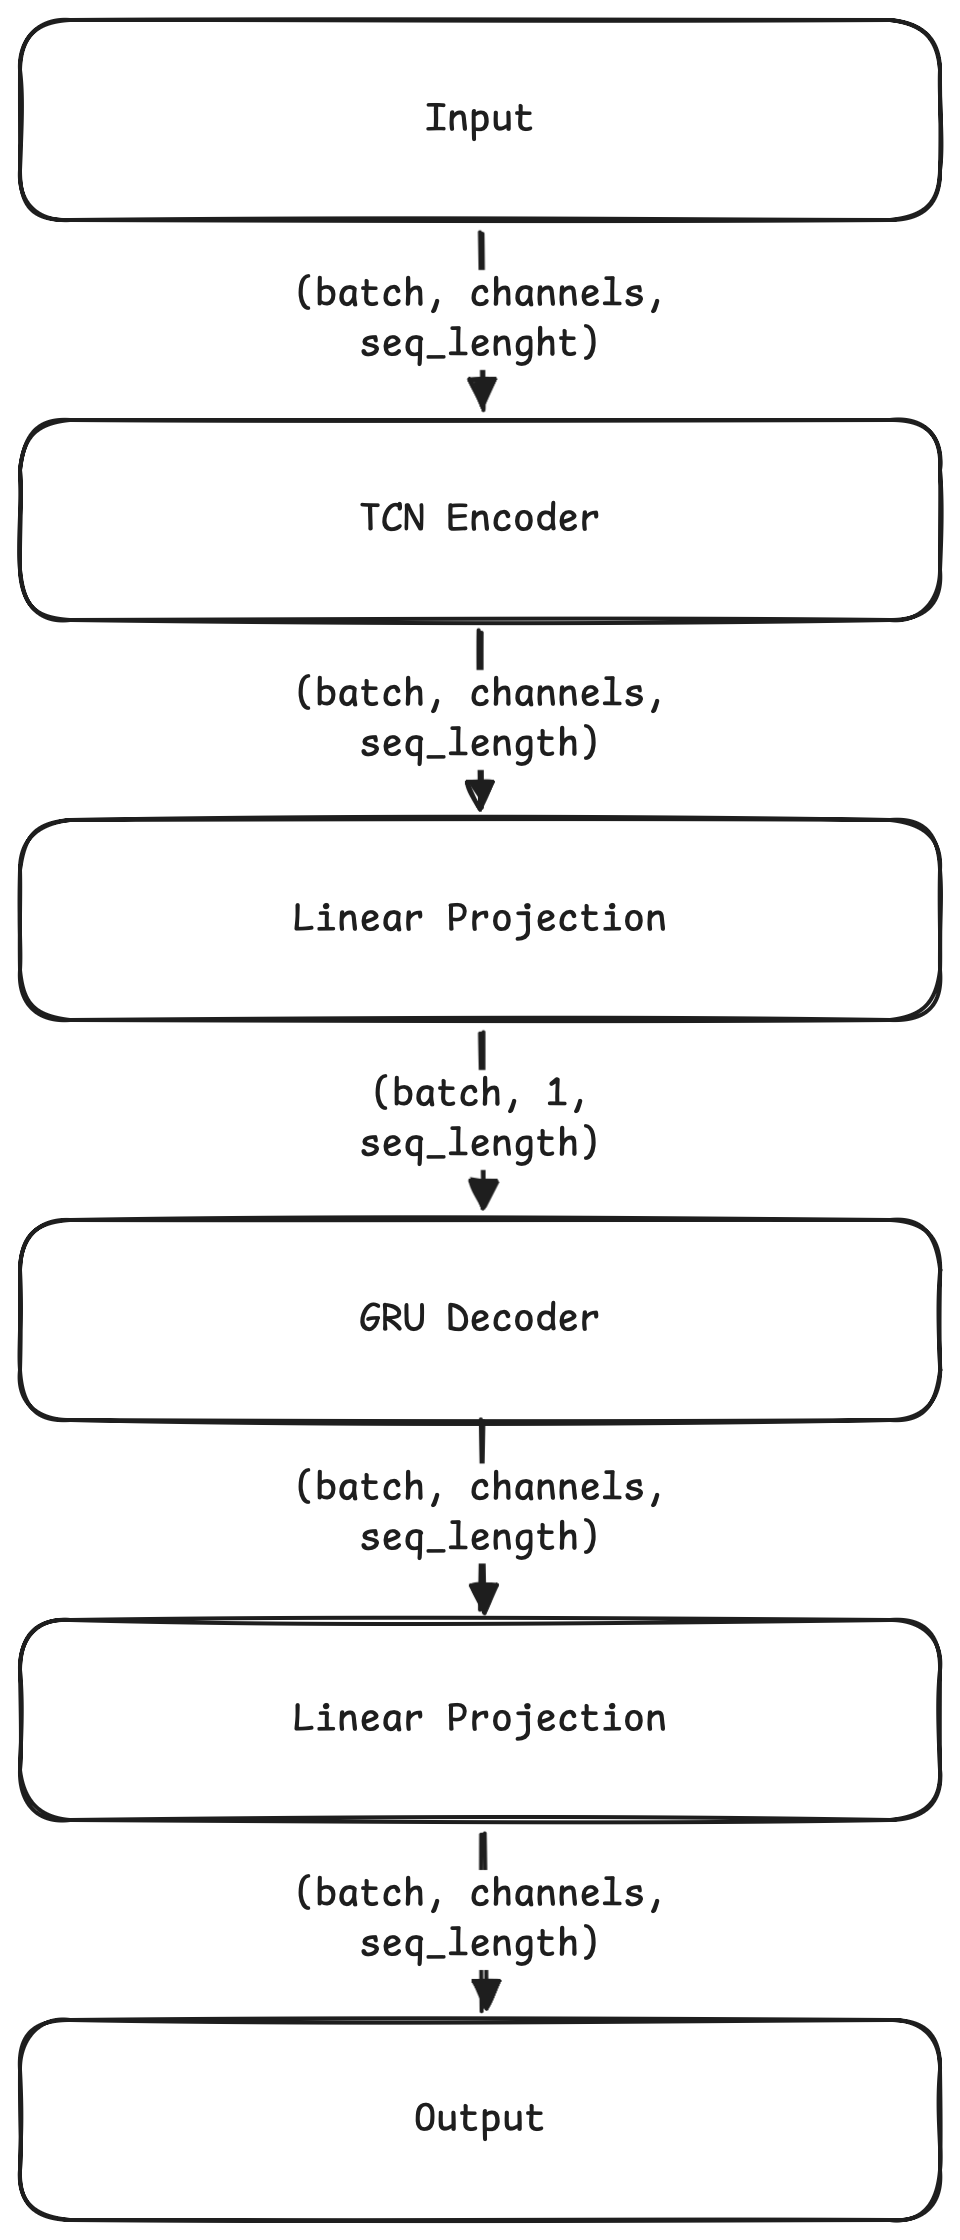
\includegraphics[width=0.40\linewidth]{figure/tcn-rnn.png}
\caption{TCN-RNN architecture} % Figure text below figure
\label{fig:tcn-rnn-architecture}
\end{figure}

The TCN encoder consists of a stack of temporal convolutional network (TCN) residual blocks with increasing dilation factors. Each TCN block is primarily composed of two causal convolutional layers, with normalization, a nonlinear activation function (ReLU), and optional dropout for regularization. Additionally, each TCN residual block implements a residual connection to stabilize training. The output is a continuous latent representation whose size is controlled by the downsampling factor and channel width. As in Zheng and Zhang~\cite{Zheng2023}, there is no downsampling in the decoder; any downsampling occurs in the linear bottleneck, which is described in the next paragraph. As a result, the input shape of the encoder is equal to its output shape. The detailed TCN encoder architecture is shown in Figure~\ref{fig:tcn-encoder}. In addition to common design choices such as dropout, residual connections, and the use of ReLU non-linearity, this encoder includes several noteworthy elements. It is designed with training efficiency and information preservation in mind. To this end, the authors use exponential dilations and additional layers to achieve stronger long-range temporal modeling. This design intentionally trades some computational efficiency for modeling capacity. The authors also employ weight normalization to improve training stability, which further increases computational cost.

\begin{figure}[h]
\centering
\subfloat[TCN encoder\label{fig:tcn-encoder}]{%
    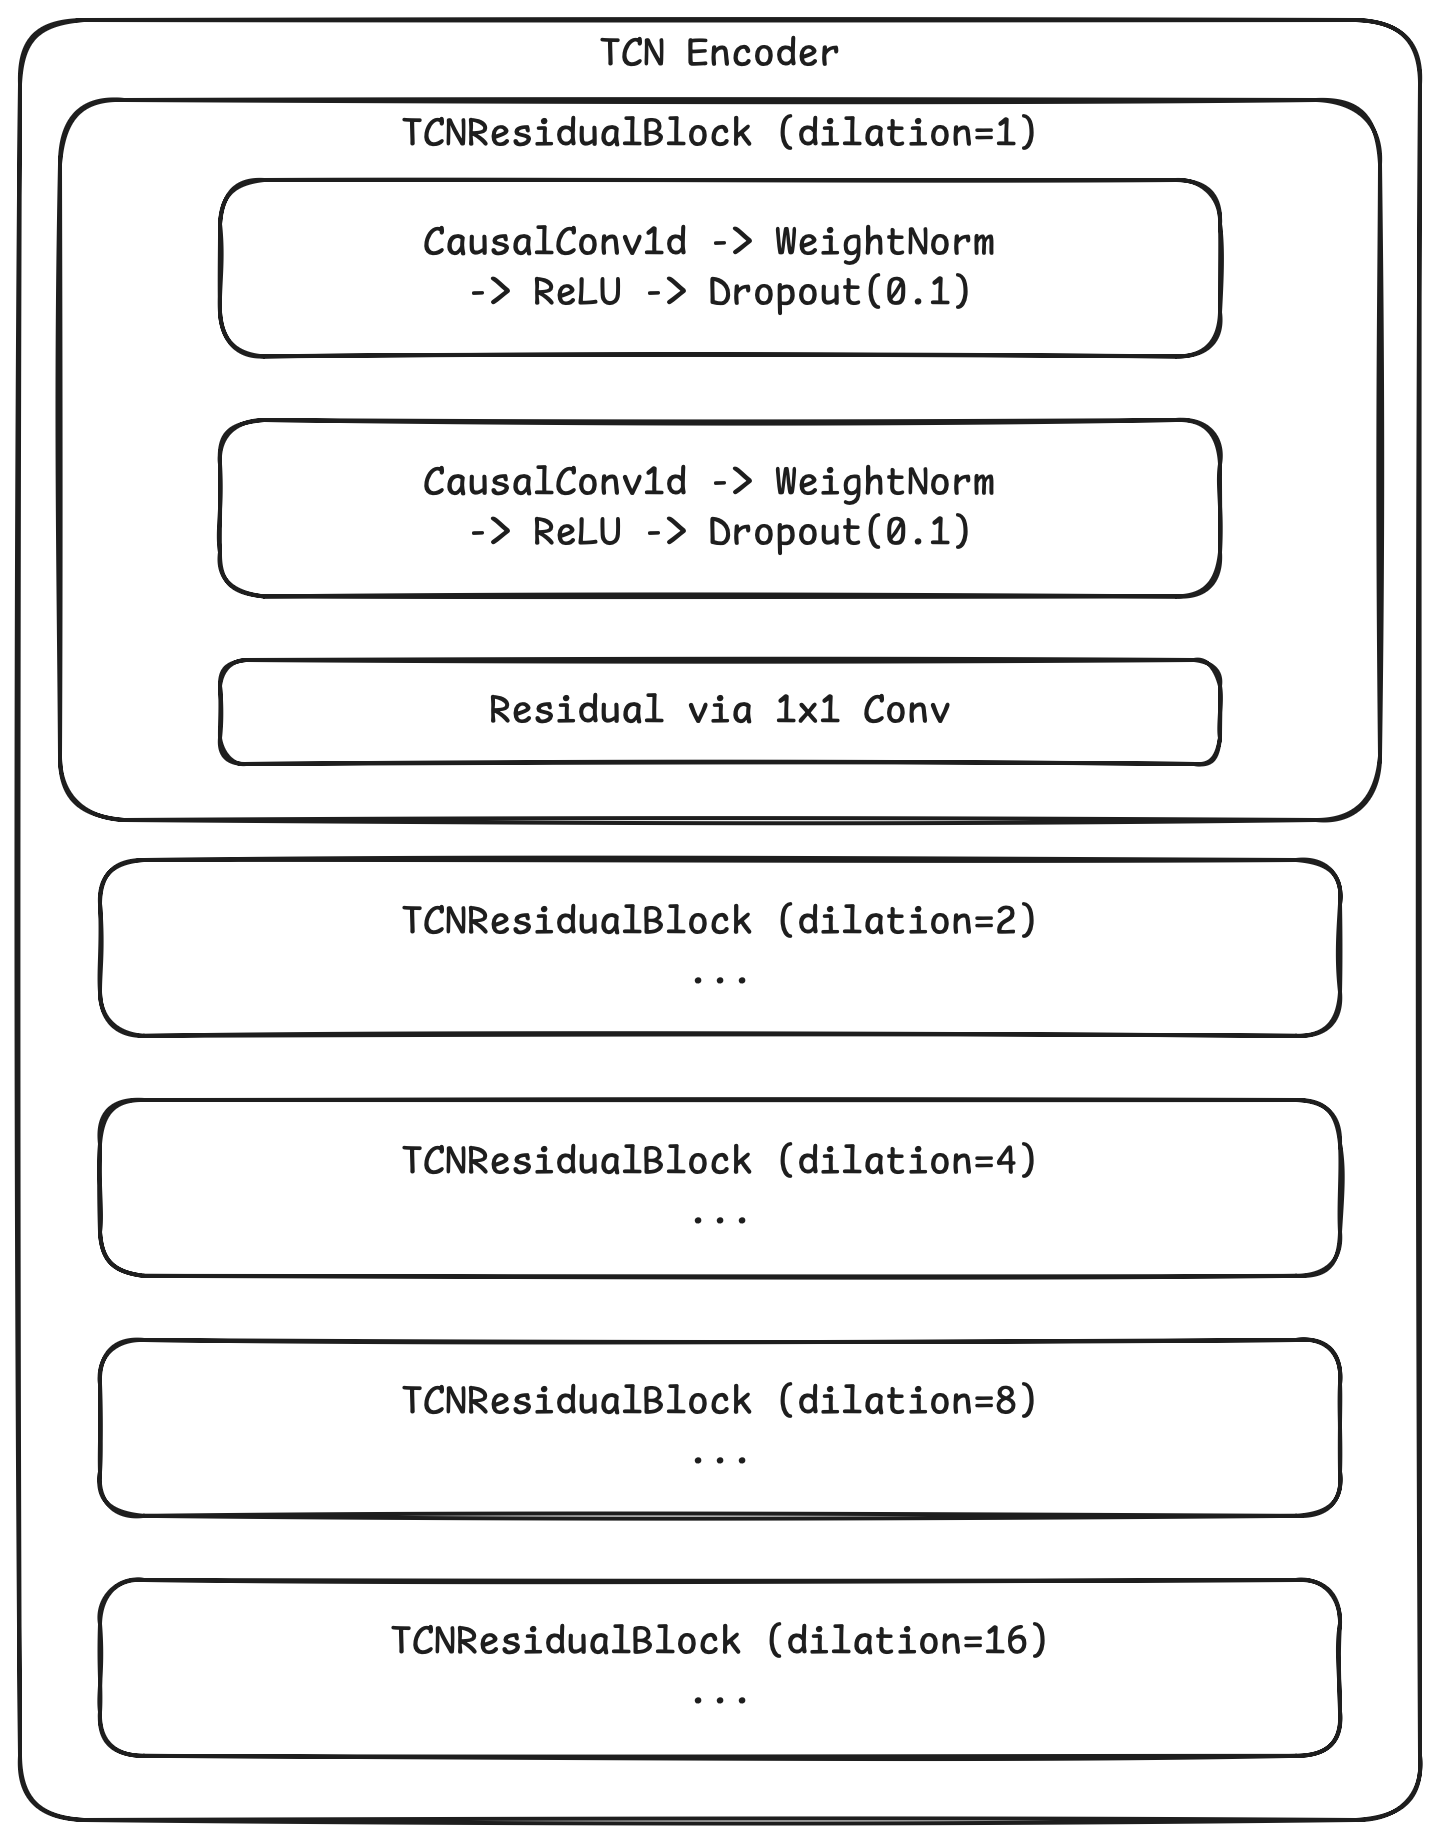
\includegraphics[width=0.48\linewidth]{figure/tcn-encoder.png}
}
\hfill
\subfloat[GRU decoder\label{fig:gru-decoder}]{%
    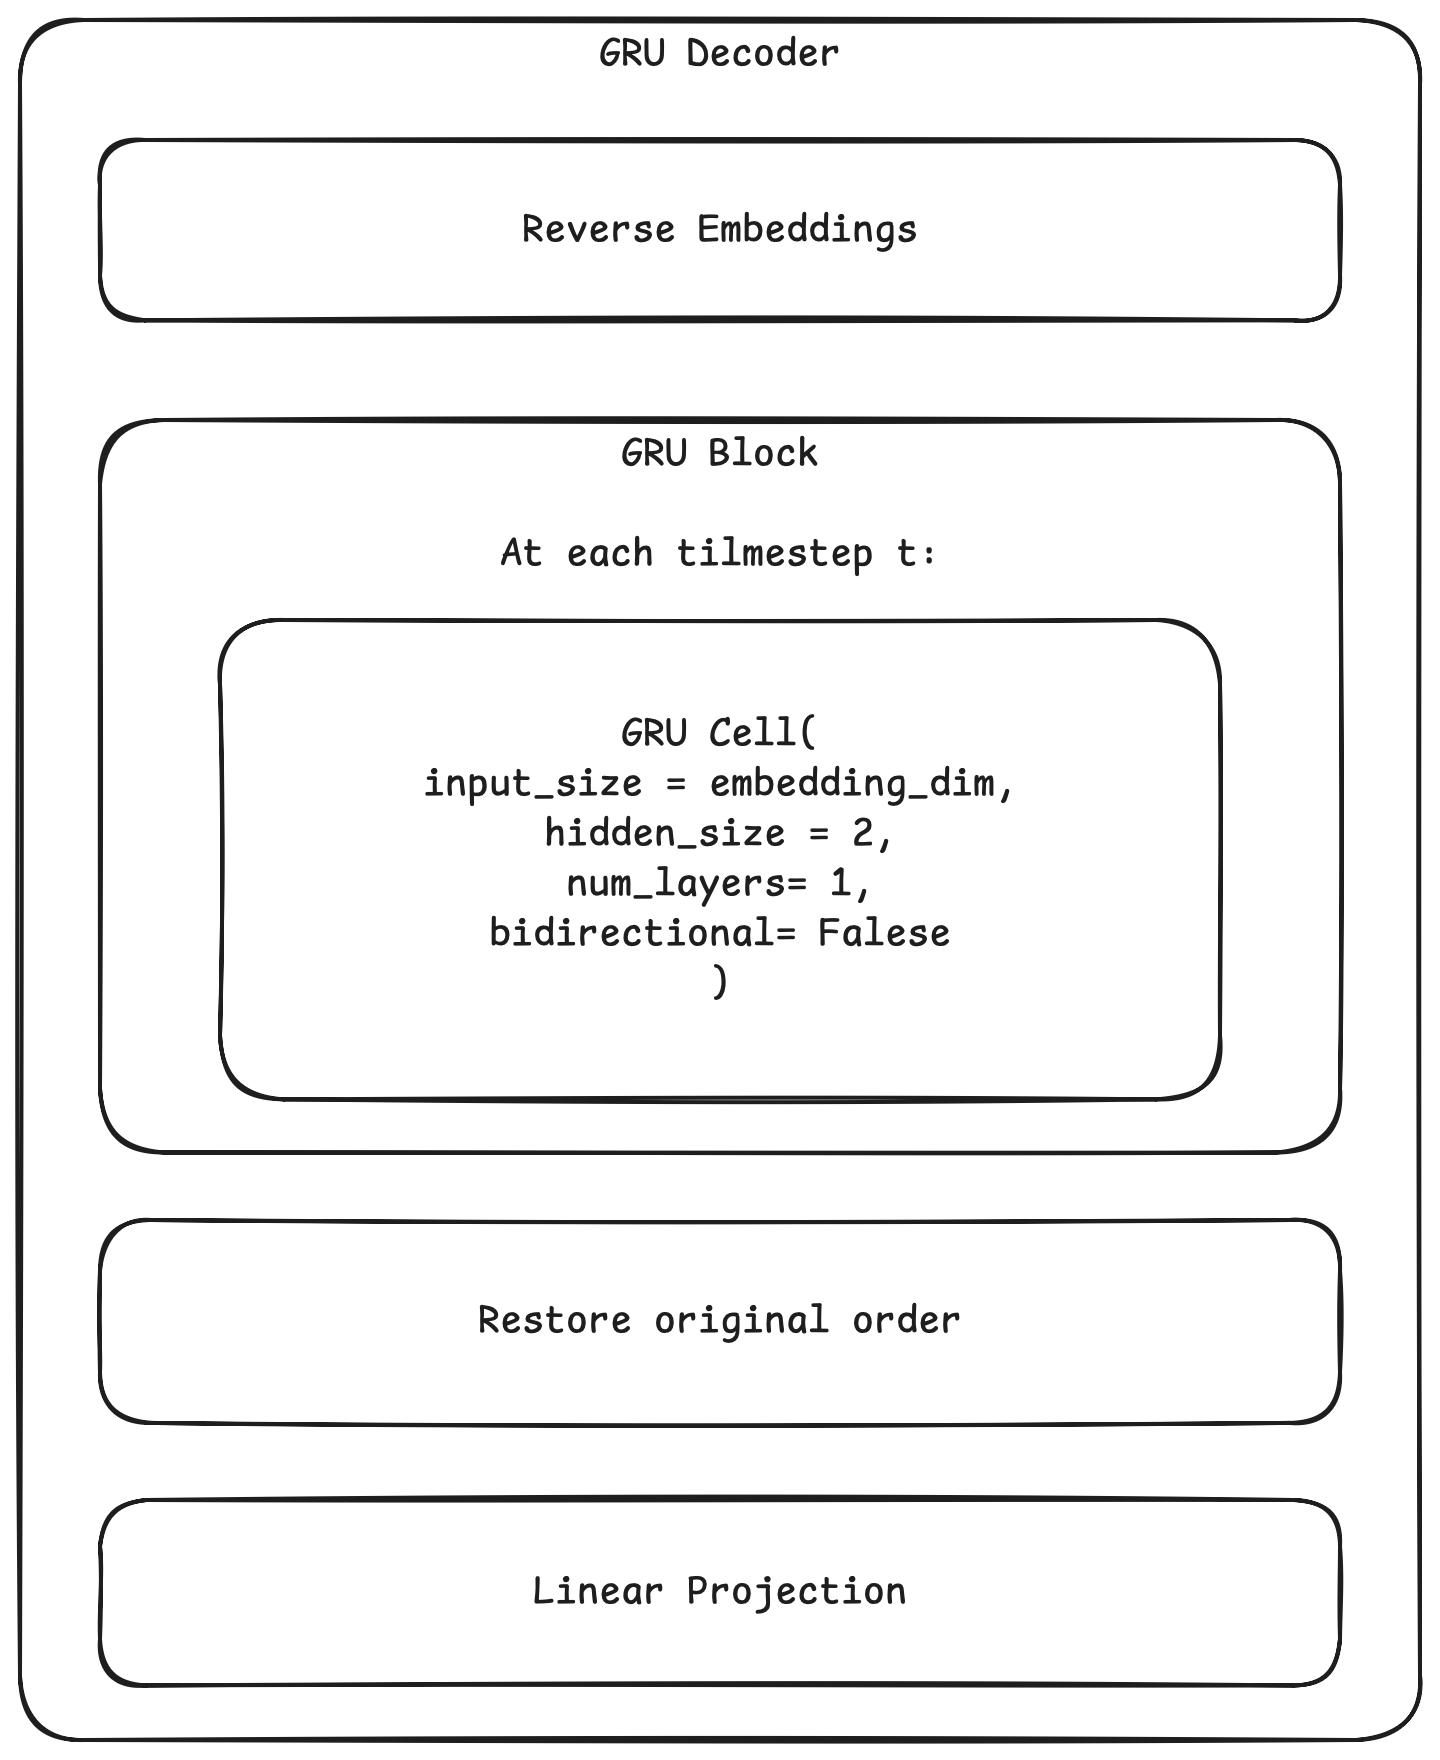
\includegraphics[width=0.48\linewidth]{figure/gru-decoder.png}
}
\caption{Detailed TCN-RNN components} % Figure text below figure
\label{fig:tcn-rnn-components}
\end{figure}

After the TCN encoder, the linear bottleneck provides the only source of geometric compression within the TCN-RNN architecture. This layer is a linear projection that reduces the input channel dimension to one. In the case of Zheng and Zhang~\cite{Zheng2023}, two input channels were used, resulting in a CR of 2:1. This means that the linear bottleneck layer of the TCN-RNN architecture produces a latent representation of the form $(\text{batch}, 1, \text{seq\_length})$.
% This is not geometric compression as we describe it above? From what I understand, geometric compression is the organization of the data in a way that allows for more effective quantization, and it importantly does not lower mutual information which a linear projection does. I'm guessing that that you are more referring to the transformation step of normal compression. (transform -> quantization -> coding). If this is the case then we should probably change the deffinition above. )

The continuous latent representation produced by the linear bottleneck serves as the input to the decoder. The decoder has two main functions. First, the embeddings are reversed for reconstruction in reverse order, meaning that the sequence is processed from end to beginning. The authors use this strategy to help the model focus on short-range temporal correlations. Second, the decoder uses a gated recurrent unit (GRU) to reconstruct the input. GRUs are a variant of RNNs that introduce reset and update gates to control the hidden state. This GRU cell expands the latent representation compressed by the bottleneck back to its original dimensionality. Afterwards, the original order is restored and a final linear projection is applied. Figure~\ref{fig:gru-decoder} shows this decoder setup in more detail.

The loss function used for the TCN-RNN baseline is identical to the loss function outlined by Zheng and Zhang~\cite{Zheng2023}. They use a simple MSE loss, but with the important caveat that they use the sum-reduced variant of MSE. The following equation shows the exact loss formula used: 

\begin{equation}
L_{\mathrm{MSE}} = \frac{1}{T} \sum_{t=1}^{T} \sum_{d=1}^{D} \left( x_t^d - \hat{x}_t^d \right)^2
\end{equation}

This function is used as the loss function for the TCN-RNN model, while the mean-reduced version of MSE is used to evaluate all the models, as described earlier in this chapter.

To validate the correctness of this implementation, a small use case from the paper is reporduced. In the paper Zheng and Zhang~\cite{Zheng2023} use the appliances energy dataset, which will be introduced at a later stage, to compress and reconstruct the two signals ``Windspeed'' and ``Appliances''. The authors present a summed MSE reconstruction error of 0.178. The implemented TCN-RNN baseline achieves a summed MSE reconstruction error of 0.133 with the same configurations, showing that it works as intended.  

\subsection{Baseline 2: EdgeCodec}

The EdgeCodec implementation leverages RVQ and a heavyweight decoder to enable a lightweight encoder architecture, which is edge-optimized~\cite{Hodo2025}. The compression mechanism of the EdgeCodec architecture is fundamentally different from the linear bottleneck employed by the TCN-RNN model. The compression achieved by EdgeCodec is a mixture of geometric compression in the encoder and compression in the information theoretic sense through quantization. The EdgeCodec encoder compresses both along the channel and the temporal axis and works as a dimensionality reduction mechanism. The quantization mechanism employed by EdgeCodec is a 4-layer hierarchical RVQ setup. The full EdgeCodec architecture is displayed in Figure~\ref{fig:edgecodec-architecture}. 

Hodo et al.~\cite{Hodo2025} provide the full code for the EdgeCodec implementation in a GitHub repository~\cite{EdgeCodec}. Therefore the EdgeCodec implementation for this thesis is largely based on this GitHub repository. An important note is that the original EdgeCodec implementation has an optional adversarial training component. For the purposes of this thesis, this is omitted, as preliminary results showed that the adversarial training component did not improve the results or was too difficult to accurately tune in the scope of this thesis. 

\begin{figure}[h]
\centering
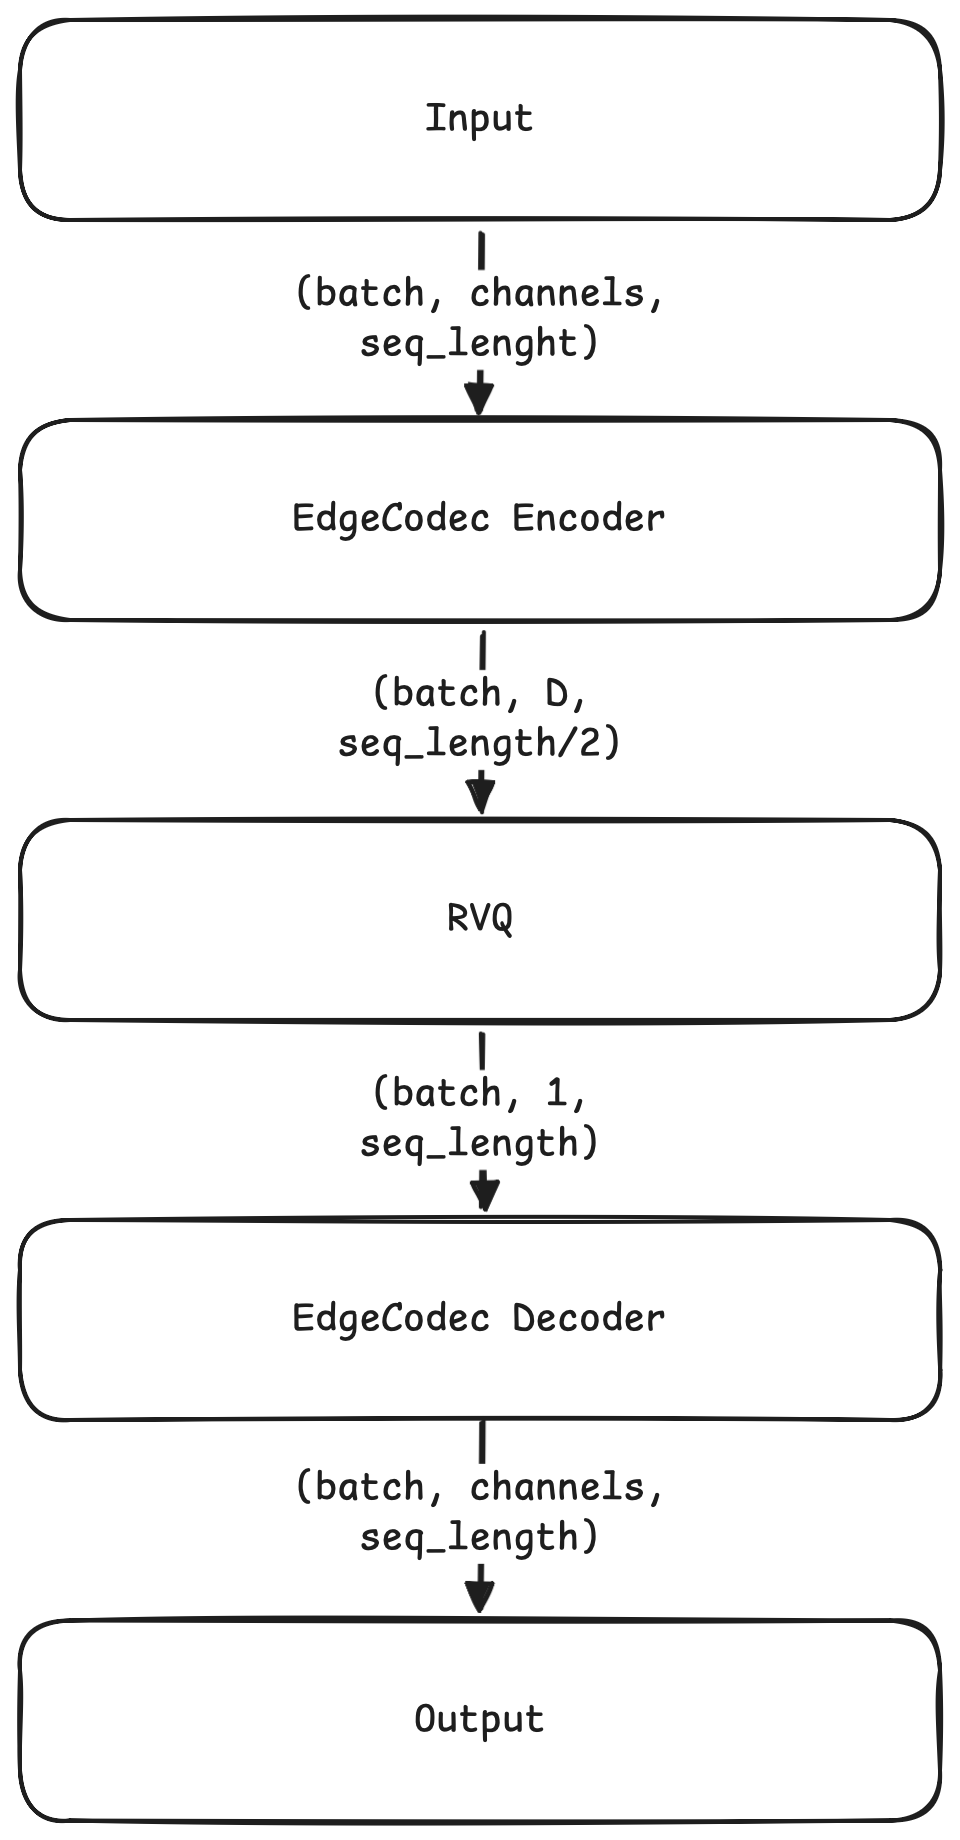
\includegraphics[width=0.40\linewidth]{figure/edgecodec.png}
\caption{EdgeCodec architecture} % Figure text below figure
\label{fig:edgecodec-architecture}
\end{figure}

The EdgeCodec encoder is intentionally lightweight. In essence, the EdgeCodec encoder architecture is fairly similar to the TCN-RNN encoder architecture. Like with the TCN-RNN encoder, the main components of the EdgeCodec encoder are residual units, which contain convolutional layers to capture local patterns. There are, however, notable differences. For one, TCN-RNN has five residual units with increasing dilation compared to the four residual units with steady dilations in the EdgeCodec encoder. Further, the EdgeCodec encoder does not use any weight normalization to optimize for computational efficiency. Another major difference between the EdgeCodec encoder and the TCN-RNN counterpart is the focus on maximizing the compression ability of the encoder. The TCN-RNN encoder employs no downsampling, neither temporal nor channel-wise. The EdgeCodec encoder actually does both. Through increasing strides, the EdgeCodec encoder is able to compress along the temporal axis, and through decreasing the input dimensionality, the EdgeCodec encoder compresses channel-wise. The CR of the EdgeCodec encoder is configurable through these two mechanisms. The detailed EdgeCodec encoder architecture with example configurations is shown in Figure~\ref{fig:edgecodec-encoder}.

\begin{figure}[h]
\centering
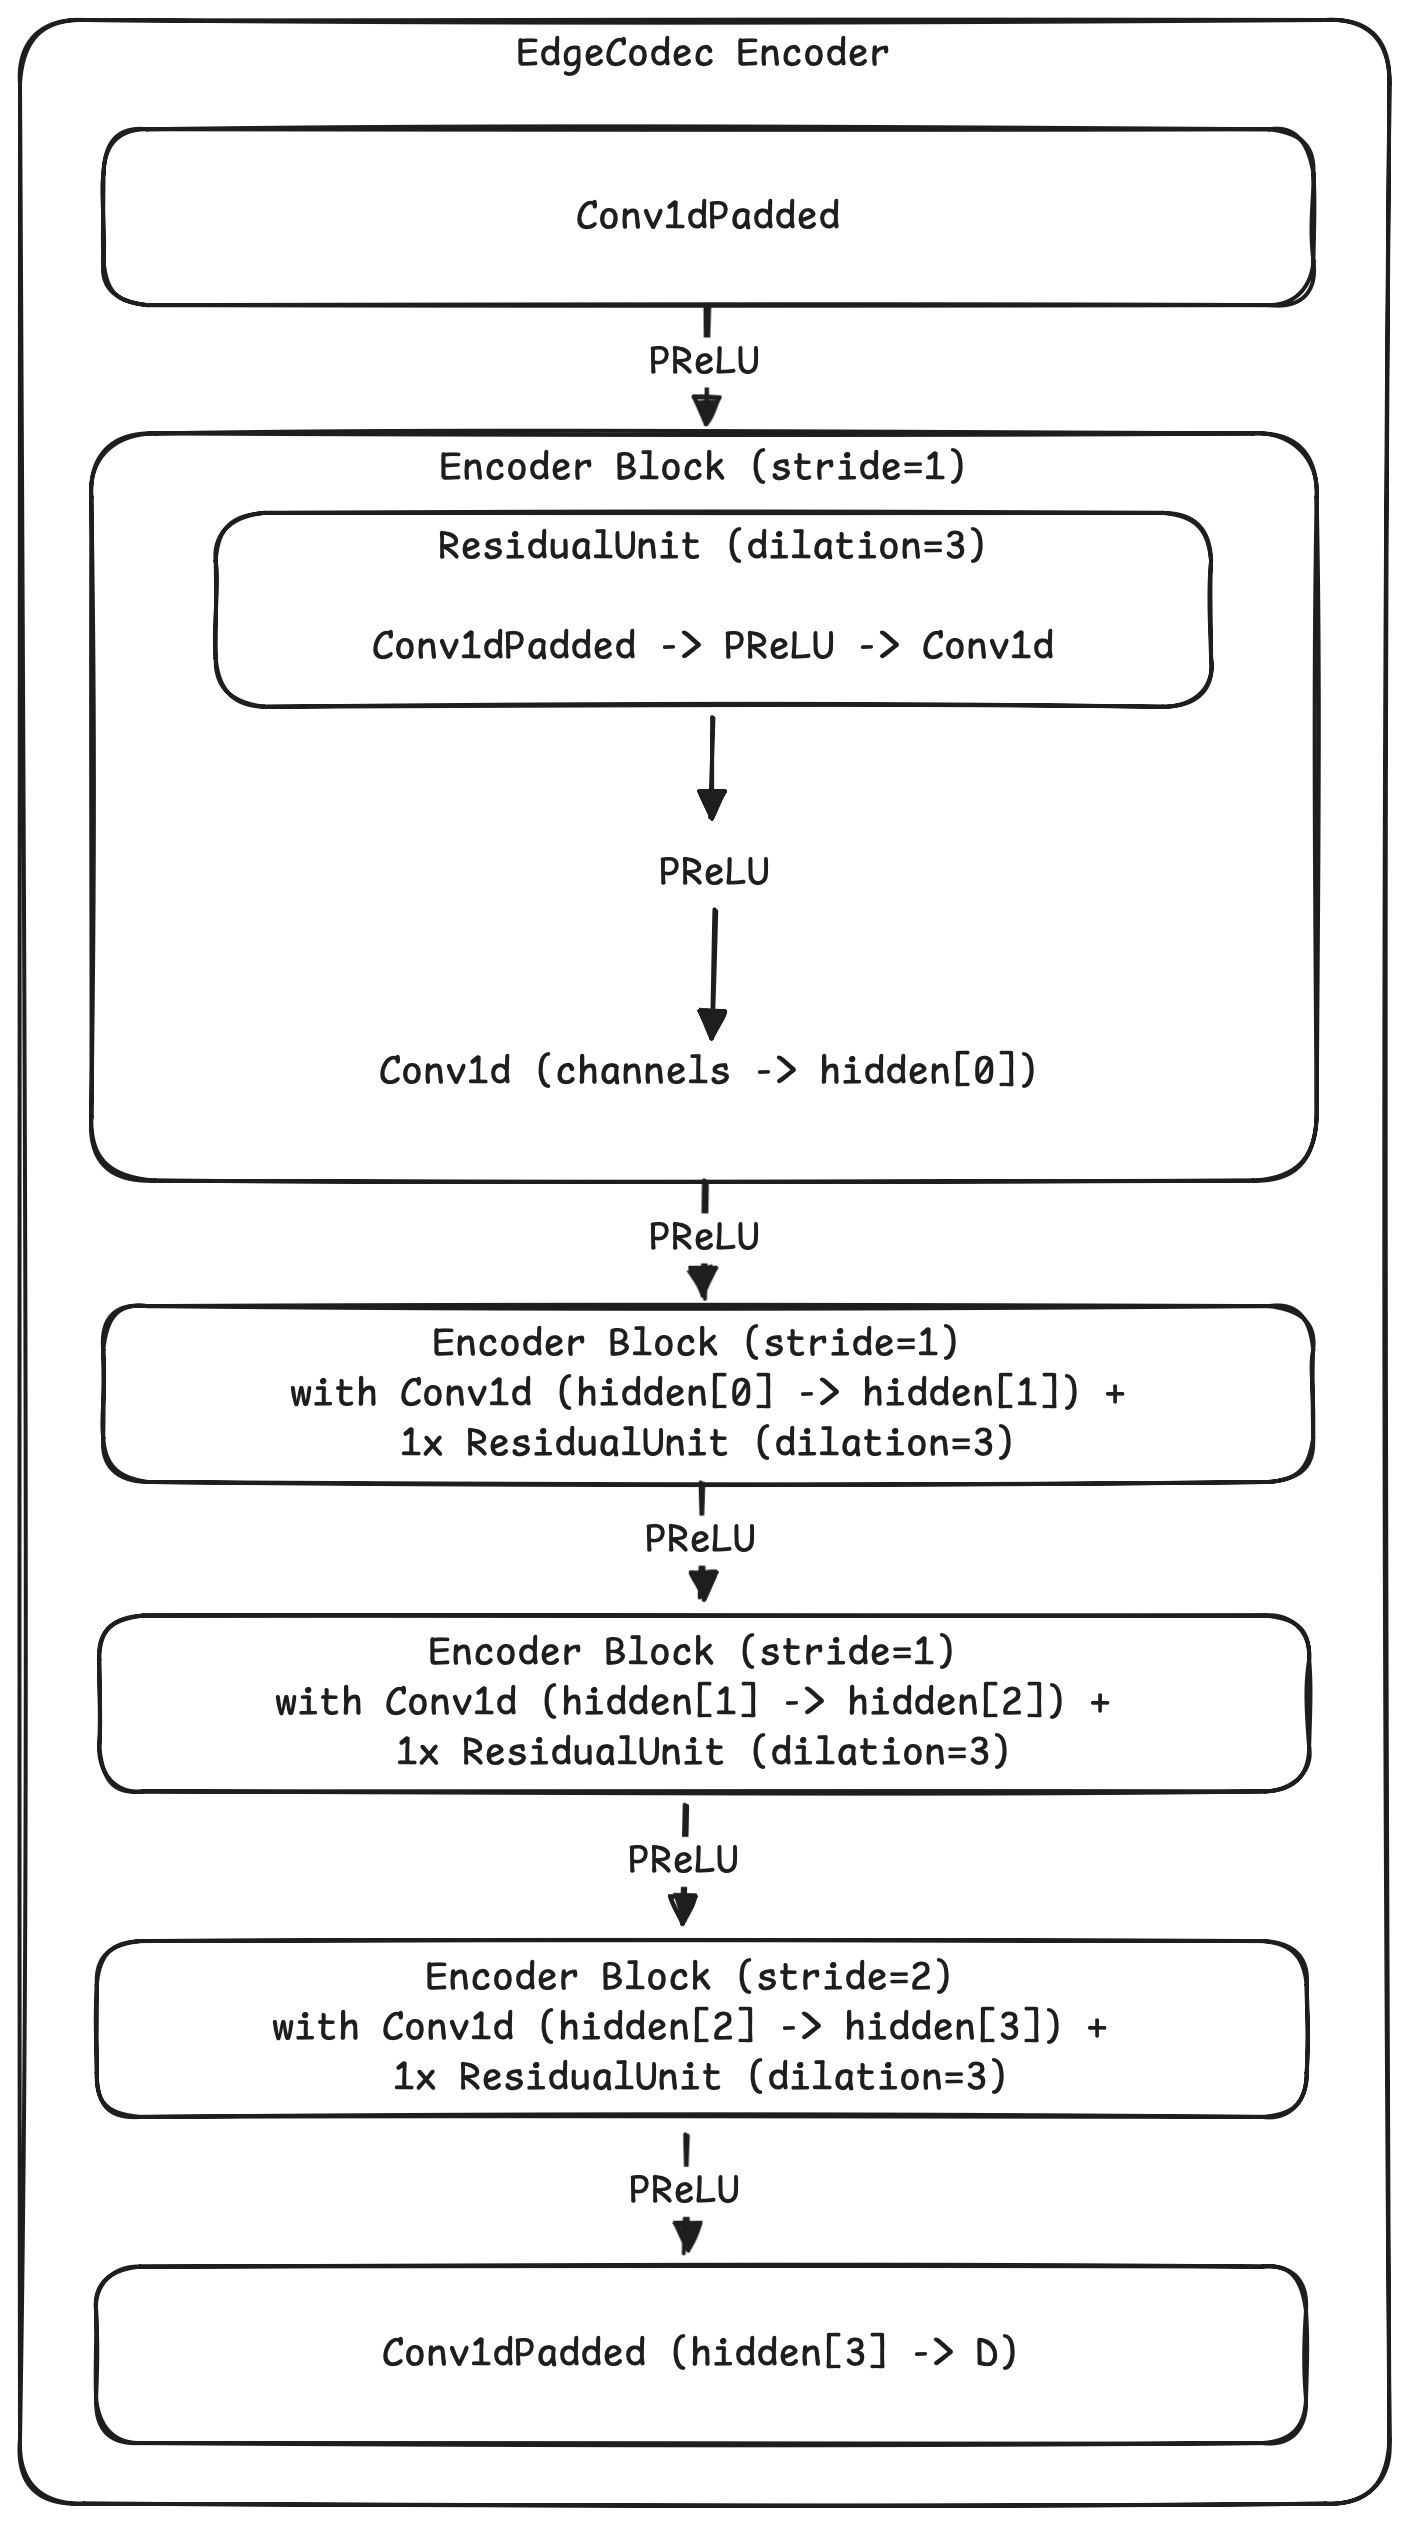
\includegraphics[width=0.40\linewidth]{figure/edgecodec-encoder.png}
\caption{EdgeCodec encoder} % Figure text below figure
\label{fig:edgecodec-encoder}
\end{figure}

Because the EdgeCodec encoder is purposefully kept lightweight, the authors compensate through a more complex and heavyweight decoder. The EdgeCodec decoder mainly implements this through channel-wise linear layers that process each channel independently. Two of these channel-wise linear layers are implemented in the EdgeCodec decoder architecture, one at the beginning and one in the middle after the first two decoder blocks. The decoder blocks are also more heavyweight compared to the encoder blocks used in the EdgeCodec encoder. Instead of only one residual unit, the decoder block implements three residual units with increasing dilation to enhance its capabilities in modeling long-range temporal patterns. The downsampling pattern along the temporal and channel-wise axis implemented in the EdgeCodec encoder is mirrored by the EdgeCodec decoder to restore the original input shape. A detailed architectural overview of the EdgeCodec decoder is presented in Figure~\ref{fig:edgecodec-decoder}.

\begin{figure}[h]
\centering
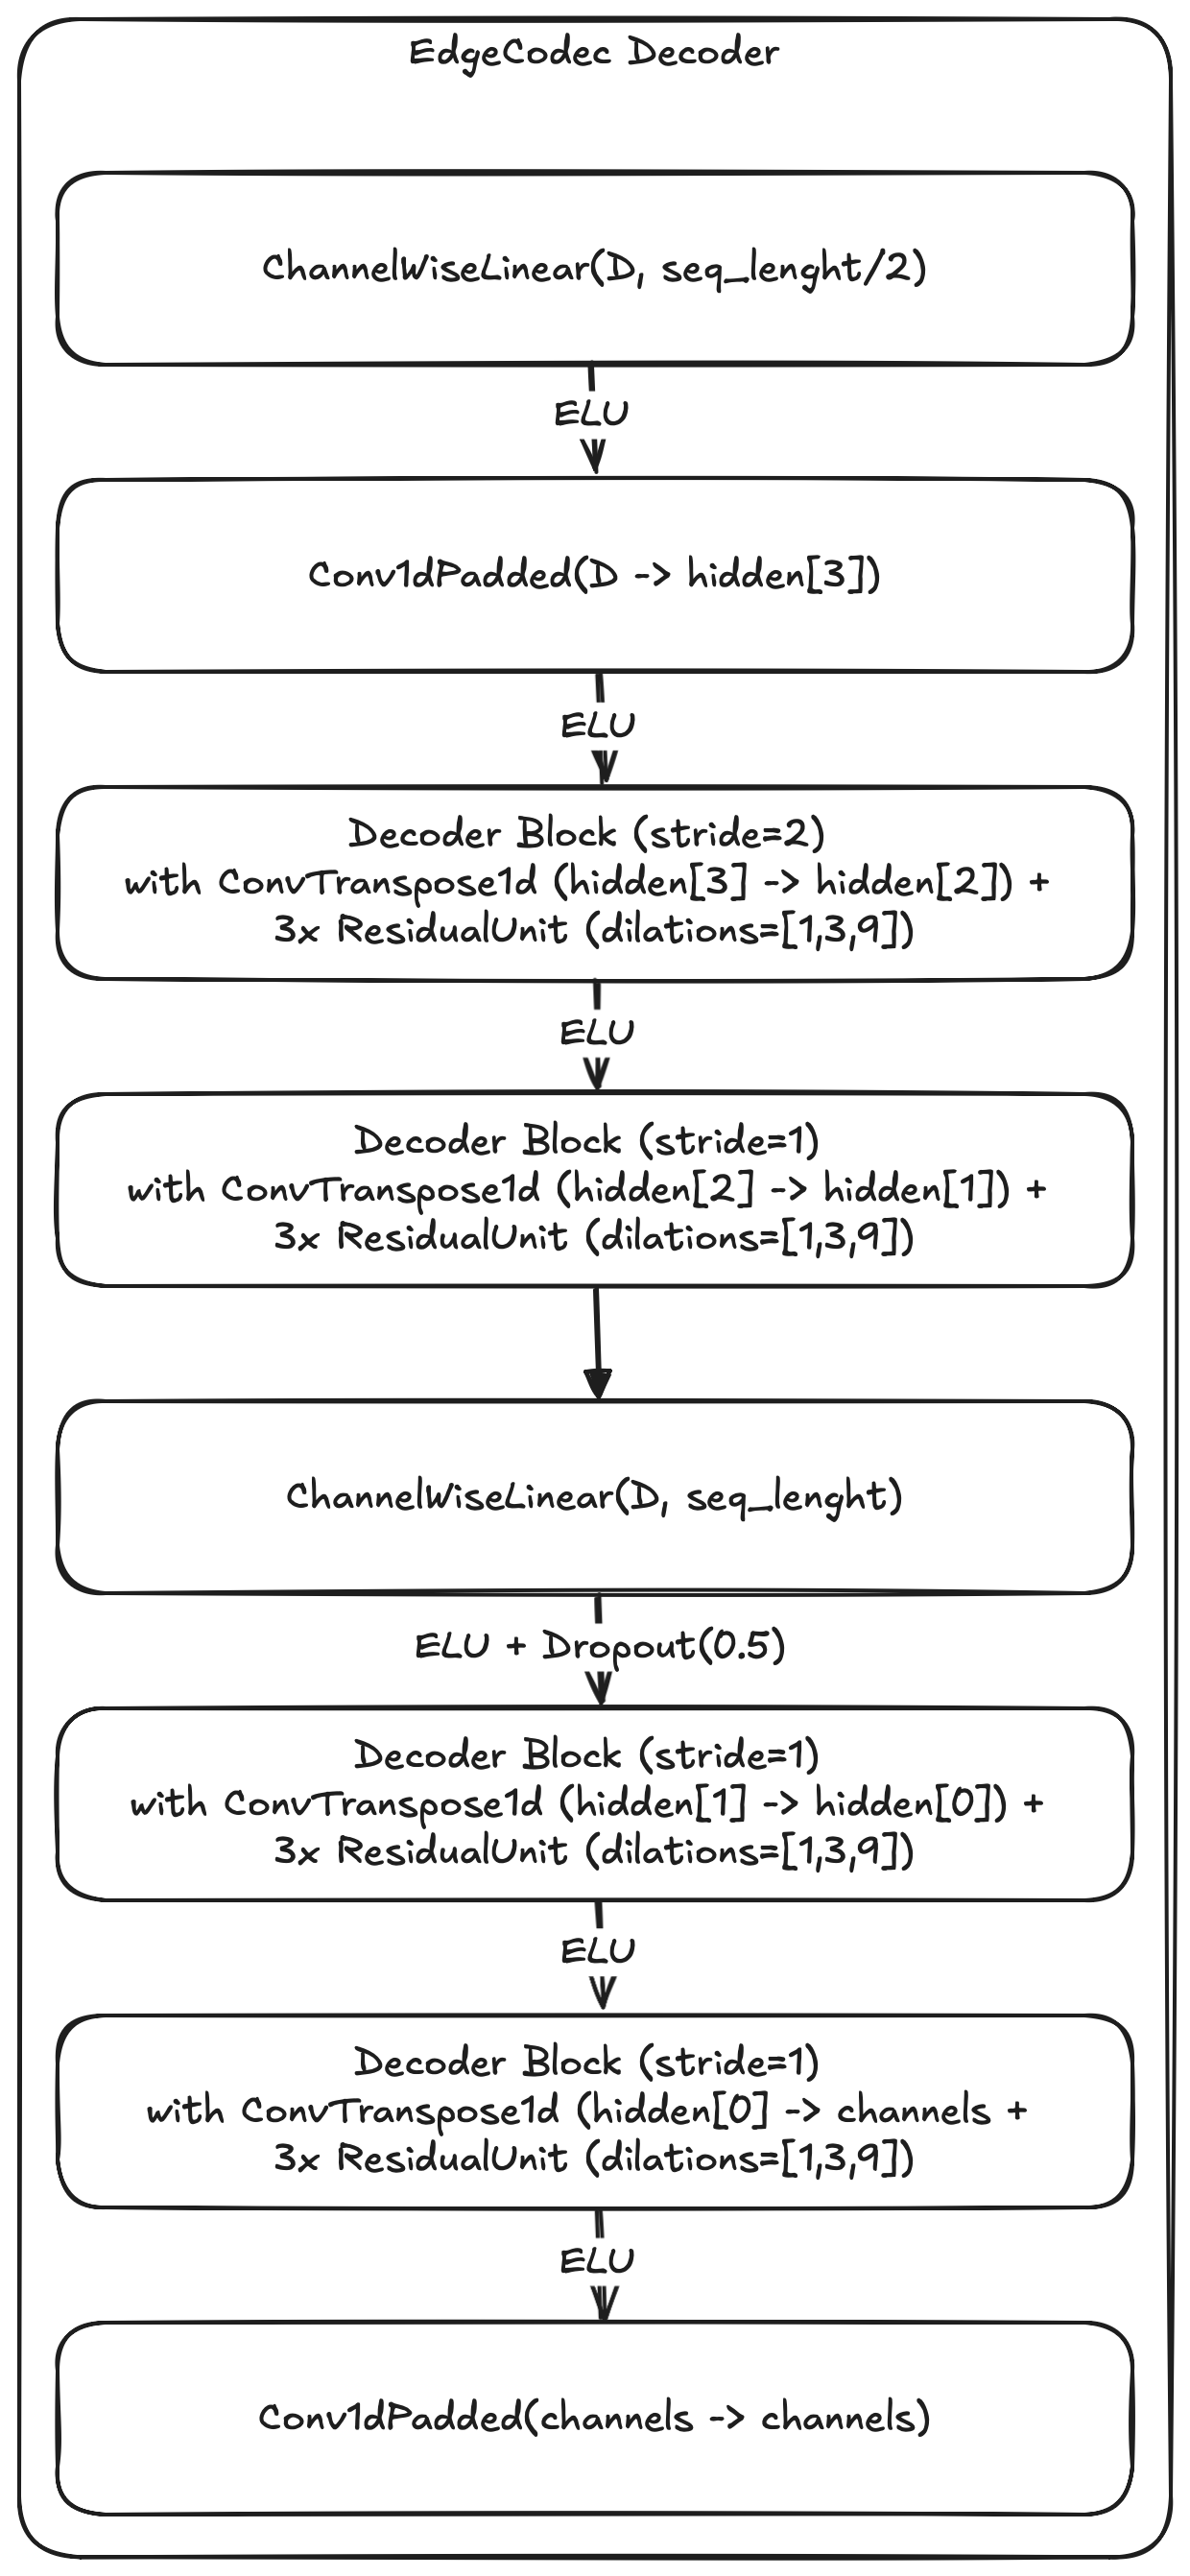
\includegraphics[width=0.30\linewidth]{figure/edgecodec-decoder.png}
\caption{EdgeCodec decoder} % Figure text below figure
\label{fig:edgecodec-decoder}
\end{figure}

Although differences in the encoder and decoder structure between the TCN-RNN and the EdgeCodec architecture are substantial, the most substantial difference between the TCN-RNN model and the EdgeCodec model is the use of a quantization mechanism to produce discrete latents. EdgeCodec utilizes a 4-level hierarchical RVQ setup to learn the codebooks. The implementation of RVQ is standardized in most modern neural compression methods through the \textit{vector-quantize-pytorch} library by Phil Wang~\cite{LucidrainsVQPT}. Hodo et al.~\cite{Hodo2025} initialize the RVQ method using embedding dimensions equal to the sequence length divided by the temporal compression of the encoder. For example, if the input has a sequence length of 128, and the encoder compresses this with a temporal CR of 2:1, the embedding dimensions for the RVQ method are 64. This enables the RVQ mechanism to assign one codebook per sequence for each channel. The non-differentiability and the resulting challenging end-to-end training of quantization methods has already been discussed above. RVQ handles this by employing exponential moving average (EMA) training, which enables more stable codebook updates compared to gradient-based training.

The loss function used to train EdgeCodec combines reconstruction error, quantization loss, and optional adversarial loss:

\begin{equation}
L(x, \hat{x}, z, \tilde{z}, y, g) = \alpha \cdot L_\mathrm{MSE}(x, \hat{x}) + (1 - \alpha) \cdot L_{l1\mathrm{-smooth}}(x, \hat{x}) + \eta \cdot L_\mathrm{RVQ}(z, \tilde{z}) + \gamma \cdot L_\mathrm{adv}(y, g)
\end{equation}

where $x$ is the input, $\hat{x}$ is the reconstructed output, $z$ and $\tilde{z}$ are the original and quantized latents, $y$ and $g$ represent the discriminator and generator outputs, and $\alpha, \eta, \gamma$ are weighting coefficients. As described before, for the purposes of this thesis, the adversarial training loss is omitted.

Because the presented implementation of the EdgeCodec baseline is heavily based on the provided code by the authors and largely reproduced one to one, an experiment to validate the correctness of this reproduction of the EdgeCodec model is omitted. 

% METHODS
% CREATED BY DAVID FRISK, 2016
\chapter{Methods}

Within this section, we will discuss the methodology employed in our project to achieve the outlined aim. Specifically, we will discuss how the architecture of the baseline established compression model and the proposed tokenization-based compression framework are designed and implemented. We additionally discuss the experiment setup we will use to compare these two approaches.

\section{Implementation Details}

\textbf{Baseline Model:} First, we want to outline the architecture of the established compression method we will use as a baseline. We will use the autoencoder approach introduced by \parencite{zheng2023} as an inspiration for our autoencoder baseline model. It is important to note, that the paper introduces a sophisticated framework consisting of two models, the TCN-RNN model and the TCN-ARNN model, as well as a model selection mechanism. For simplicity sake, we will only focus on one of these models, the TCN-RNN model. The TCN-RNN model described in the paper is a representative of state-of-the-art continuous-latent neural time-series compression methods. Compared to vanilla autoencoders, the models architecture is explicitly designed for long temporal dependencies and has demonstrated stronger rate-distortion performance. This allows us to evaluate our tokenization-based approach against a competitive neural compressor rather than a toy model. Another point to note about the TCN-RNN model, is its costly architectural design, namely deep temporal convolutional stacks with large receptive fields, recurrent (often sequential) decoding, and dense continuous latent representations. These components typically lead to increased FLOPs, higher activation memory, and longer inference latency compared to discrete, token-based compression methods.

On a high level, the TCN-RNN architecture consists of the following components:

\begin{itemize}
    \item Input handling and preprocessing
    \item TCN encoder
    \item RNN bottleneck 
    \item RNN decoder
    \item TCN decoder 
\end{itemize}

For the input handling and preprocessing it is important that the time-series data is segmented into fixed-length windows. These windows are treated as inputs to the model. Overlapping windows can be used to increase the effective training data size and improve reconstruction quality at window boundaries. Additionally, each channel is normalized independently using statistics computed on the training set.

The TCN encoder consists of a stack of Temporal Convolutional Network (TCN) blocks with increasing dilation factors. Each TCN block contains: A 1D convolution operating along the temporal dimension, normalization (BatchNorm or LayerNorm), a nonlinear activation function (ReLU or LeakyReLU), optional dropout for regularization, and a residual connection to stabilize training. The outcome is a continuous latent representation whose size is controlled by the downsampling factor and channel width.

The encoder output is processed by a recurrent neural network, specifically a gated recurrent unit (GRU), the RNN bottleneck. The RNN captures longer-range temporal dependencies that are not easily modeled by convolutions alone. At this stage, we produce a sequence of hidden states that serves as the core compressed signal. The hidden state dimensionality and number of layers define the strength of the bottleneck. The compression is achieved implicitly by restricting temporal resolution and latent dimensionality rather than by discretization. Afterwards, the RNN decoder reconstructs a latent sequence from the bottleneck representation. The decoder mirrors the bottleneck RNN in depth and hidden size.

Finally, a mirrored TCN stack upsamples the latent sequence back to the original temporal resolution. Transposed convolutions or interpolation-based upsampling are used. A final linear projection maps features back to the original channel dimension. The overall training objective is the reconstruction loss (e.g., MSE or MAE) between input and reconstructed signal.

\textbf{Tokenization-Based Compression Framework:} Next, we outline the architecture of our proposed tokenization-based compression framework. The architecture is inspired by recent advances in neural compression for speech and audio data, namely the Wavtokenizer paper. The key idea is to replace continuous latent representations with discrete tokens drawn from a learned codebook. 

We again want to first outline the high-level components of the architecture:

\begin{itemize}
    \item Input handling and preprocessing
    \item Lightweight encoder
    \item Vector quantization / tokenization
    \item Decoder head (for reconstruction) or downstream head (for task-specific loss)
\end{itemize}

The first component is (and should be) identical to the TCN-RNN baseline model. This ensures that any performance differences can be attributed to the compression method rather than preprocessing variations. 

The encoder layer functionally has the same goal s the TCN encoder used in the baseline model, but has a different architecture. The encoder is designed to be lightweight, avoiding heavy temporal convolutions or recurrent layers. Instead, a shallow neural network (e.g., small CNN or MLP applied per timestep) maps the input signal to intermediate embeddings. The encoder implements the learned transform stage of a lossy compression pipeline. Its purpose is not to predict labels or reconstruct the input per se, but to reshape the data into a representation that can be efficiently discretized. Specifically, the encoder learns a mapping that removes redundancy and correlations present in the raw time series, concentrates important information into a low-dimensional, stable representation, and aligns the geometry of the representation space with the constraints of quantization. The objective is usually joined with the quantization and decoder stages.

In contrast to autoencoder-based methods, where the encoder is free to produce high-entropy continuous latents, the encoder here is explicitly shaped to produce quantization-friendly representations that support discrete tokenization and entropy coding.

The next component is the vector quantization / tokenization stage. Here, intermediate embeddings are discretized using a learned codebook. The codebook very simply looks like this: codebook = nn.Parameter(torch.randn(K, D)), with K = number of tokens and D = embedding dimension. Each embedding vector is replaced by the index of its nearest codebook entry. This step introduces the only explicit source of information loss. The output is a sequence of discrete token IDs drawn from a finite vocabulary.

Lastly, we implement a head to enable loss calculation and backpropagation. Depending on the use case, this head can be a decoder for reconstruction tasks or a downstream head for task-specific losses (e.g., classification or regression). The head architecture is flexible and can be adapted to the specific application. The calculated loss is then used to jointly optimize the encoder, codebook, and head parameters.

\section{Experiment Setup}

To compare and evaluate the two methods outlined above, we will conduct a series of experiments. In this subsection we outline how we ensure a fair comparison, what metrics we will use, and what data we will use for the experiments.

\textbf{Comparison and Metrics:} There are three dimensions along which we want to compare the two compression methods. First, we want to evaluate the \textit{compression performance} of both methods. This includes the metrics compression rate and reconstruction error. These metrics align with the evaluation standards in the neural compression literature. We will measure these metrics by training the two models on a reconstruction task and evaluating the reconstruction quality and effective compression rate. Second, we want to evaluate the \textit{downstream task performance} when using compressed representations from both methods. This includes metrics such as accuracy for classification tasks or mean squared error for regression tasks. This evaluation reflects the practical utility of the compressed data for real-world applications. Third, we want to compare the \textit{model efficiency} of both methods. This includes metrics such as parameter count, computational cost (FLOPs), inference latency, and memory footprint. These metrics are important for assessing the feasibility of deploying the compression methods in resource-constrained environments.

An important note to make regarding comparability of these two metrics, especially regarding the downstream task performance, is that the two methods produce different types of compressed representations. The TCN-RNN baseline produces a continuous latent representation and the tokenization-based method produces discrete tokens. To ensure a fair comparison, we will need to design a lightweight unobtrusive adapter for each representation type that maps them into a common format suitable for the downstream model. The adapters should have minimal capacity to avoid introducing bias. This way, we can isolate the effect of the compression method itself on downstream performance. The envisioned design for the adapters is as follows:

\begin{itemize}
    \item The adapter for the continuous latent representation will take the sequence of real-valued vectors output by the TCN-RNN model, average them over time to produce a single vector, and then pass this vector through a linear layer to match the input size of the downstream model.
    \item The adapter for the token-based representation will take the sequence of token IDs output by the tokenization model, map each token ID to a small vector using an embedding lookup, average these embeddings over time to produce a single vector, and then pass this vector through a linear layer to match the input size of the downstream model.
\end{itemize}

\textbf{Data:} The goal is to use industry relevant data, while also ensuring that the methods are tested on publicly available data. For that reason, we will use three datasets: Two Volvo datasets, the Volvo test fleet dataset and the Volvo electric mobility (EMOB) dataset, and a third publicly available dataset called X-CANIDS \parencite{JeongLLK24X-CANIDS}. Each of these datasets contains multivariate time-series data collected from vehicles, including sensor readings, telemetry data, and operational parameters. The test fleet dataset will be used to construct a downstream regression task focused on predicting a continuous target variable. The EMOB dataset will be used to construct a downstream classification task, namely anomaly detection in battery systems. The publicly available dataset will be used as an additional benchmark to validate the generalizability of the findings across different data sources.

\textbf{Downstream Models:} Comparing the compression methods based on downstream task performanc requires downstream models. These models need to be simple enough to let us easily evaluate the compression methods used to compress the data which is fed into these models, but also still relevant to actual use cases. For this reason we will use four different downstream models to test the capabailities of the described compression methods. First, we will use the Volvo datasets to creat a regression (fuel consumption) and a classification (anomaly detection) downstream model. Second, we will use the X-CANIDS dataset to again create two models, one regression and one classification. 

% RESULTS
% CREATED BY DAVID FRISK, 2016
\chapter{Experimental Results}

Within this chapter the results of the experiments are presented. The results are presented in order of importance, starting with the key findings and then comparing each neural compression method per metric. 

\section{Key Findings}

Top-line result: one clear sentence naming the best model and the primary metric (value + CI).
Secondary wins: 1–2 bullets for notable trade-offs or dataset-specific wins.
Major negative / surprise: 1 bullet about what underperformed or an unexpected result.
Practical implication: 1 sentence about which model(s) to prefer for specific use-cases.
Link to figures: short pointers to the supporting table/plot numbers.

\section{Comparative Evaluation}

The two dimensions along wich each of the neural compression methods are evaluated are compressione performance and downstream task performance, as outlined in Chapter~\ref{chap:methods}. In the results for all neural compression methods for all datasets across both these dimensions are presented. 

\subsection{Compression Performance}

\subsection{Downstream Task Performance}





% CONCLUSION
% CREATED BY DAVID FRISK, 2016
\chapter{Conclusion}

\section{Discussion}

Mechanistic explanations (why a model won).
Broader implications and recommendations beyond immediate use-cases.
Limitations, theoretical interpretation, future work.

\section{Conclusion}


% REFERENCES / BIBLIOGRAPHY
\clearpage
\phantomsection % So hyperref does not link to the section above
\addcontentsline{toc}{chapter}{Bibliography}
\printbibliography

% APPENDICES
\clearpage
\appendix
\setcounter{page}{1}
\pagenumbering{Roman}			% Capitalized roman numbering starting from I (one)

% CREATED BY DAVID FRISK, 2016
\chapter{Appendix}

\section*{Complete Empirical Results}
\label{app:empirical-results}

The code and complete empirical results for all models and datasets are available at https://github.com/TimBoleslawsky/neural-compression-thesis under the directory /results.


\end{document}